\chapter{Simulación en Geant4.}

De acuerdo a las propiedades de los morteros, estos son construidos en Geant4 y se procede a hacer las simulaciones correspondientes. 

\section{Transmisión.}

Las energías utilizadas son (picos de izquierda a derecha) 81 keV, 122 keV, 356 keV, 511 keV, 662 keV, 1173 keV, 1273 keV y 1332 keV. Se hace la simulación con estas ya que en el laboratorio se tienen fuentes de  $^{137}Cs$, $^{133}Ba$, $^{60}Co$, $^{57}Co$ y $^{22}Na$, estas emiten fotones a las energías mencionadas.
  
\begin{figure}[H]
	\centering
	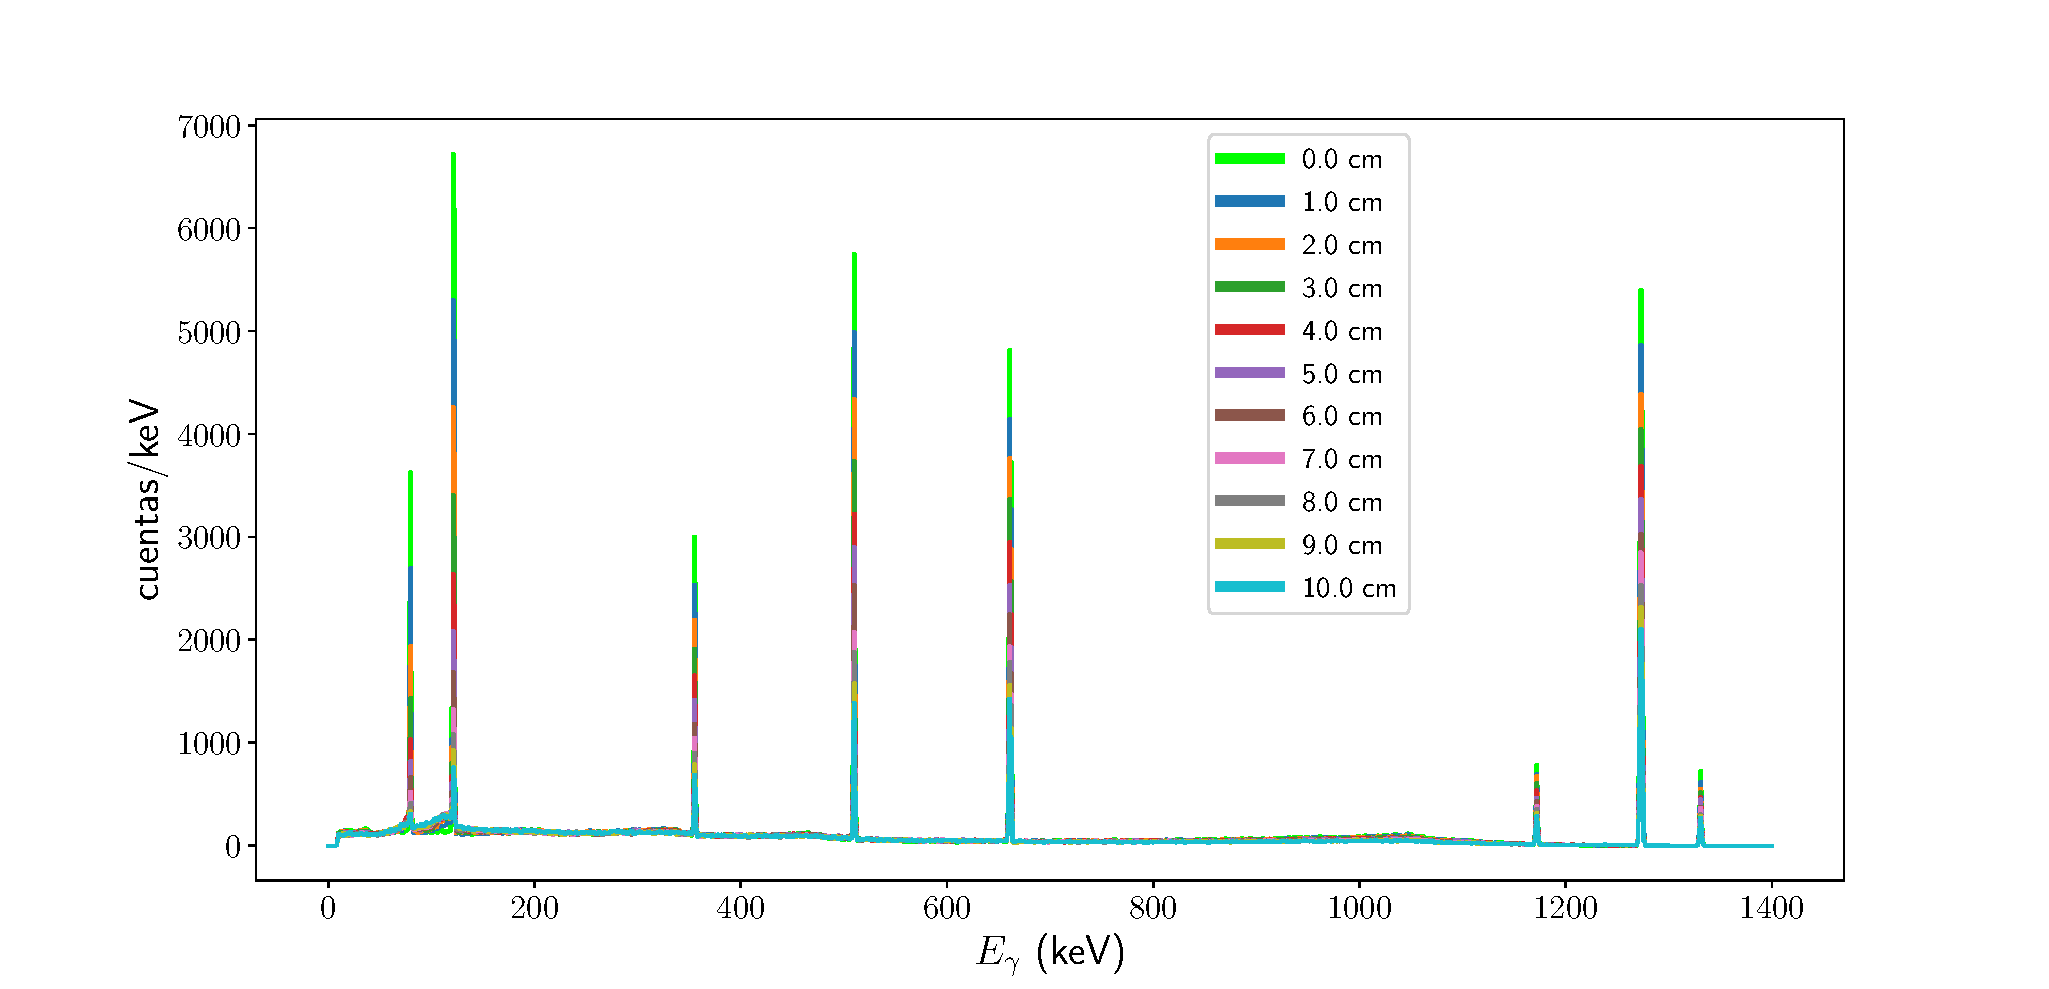
\includegraphics[width=0.8\linewidth]{Kap4/espectro_m1-10M-trans.pdf}
	\caption{Espectro de 10 láminas de Morteros1. Transmisión}
	\label{fig:espectrom1-10m-trans}
\end{figure}


Como se puede ver, cuanto mas grueso el material, la intensidad máxima disminuye. Esto se debe a que obedece la ecuación \ref{intensidad}. 

\begin{equation}\label{intensidad}
    I=I_0e^{-\mu x}
\end{equation}


donde $I_0$ es la intensidad inicial, $\mu$ el coeficiente de atenuación y $x$ el grosor del material. Esta ultima es la variable, en el presente texto será llamada $t$. El valor de $\mu$ es encontrado para cada fotopico. Es fácil ver que se tendrán 8 valores. Con estos se hace un ajuste de la forma:

\begin{equation}
	\frac{\mu}{\rho}=\alpha\times E^{-n}.
\end{equation}

\begin{figure}[H]
	\centering
	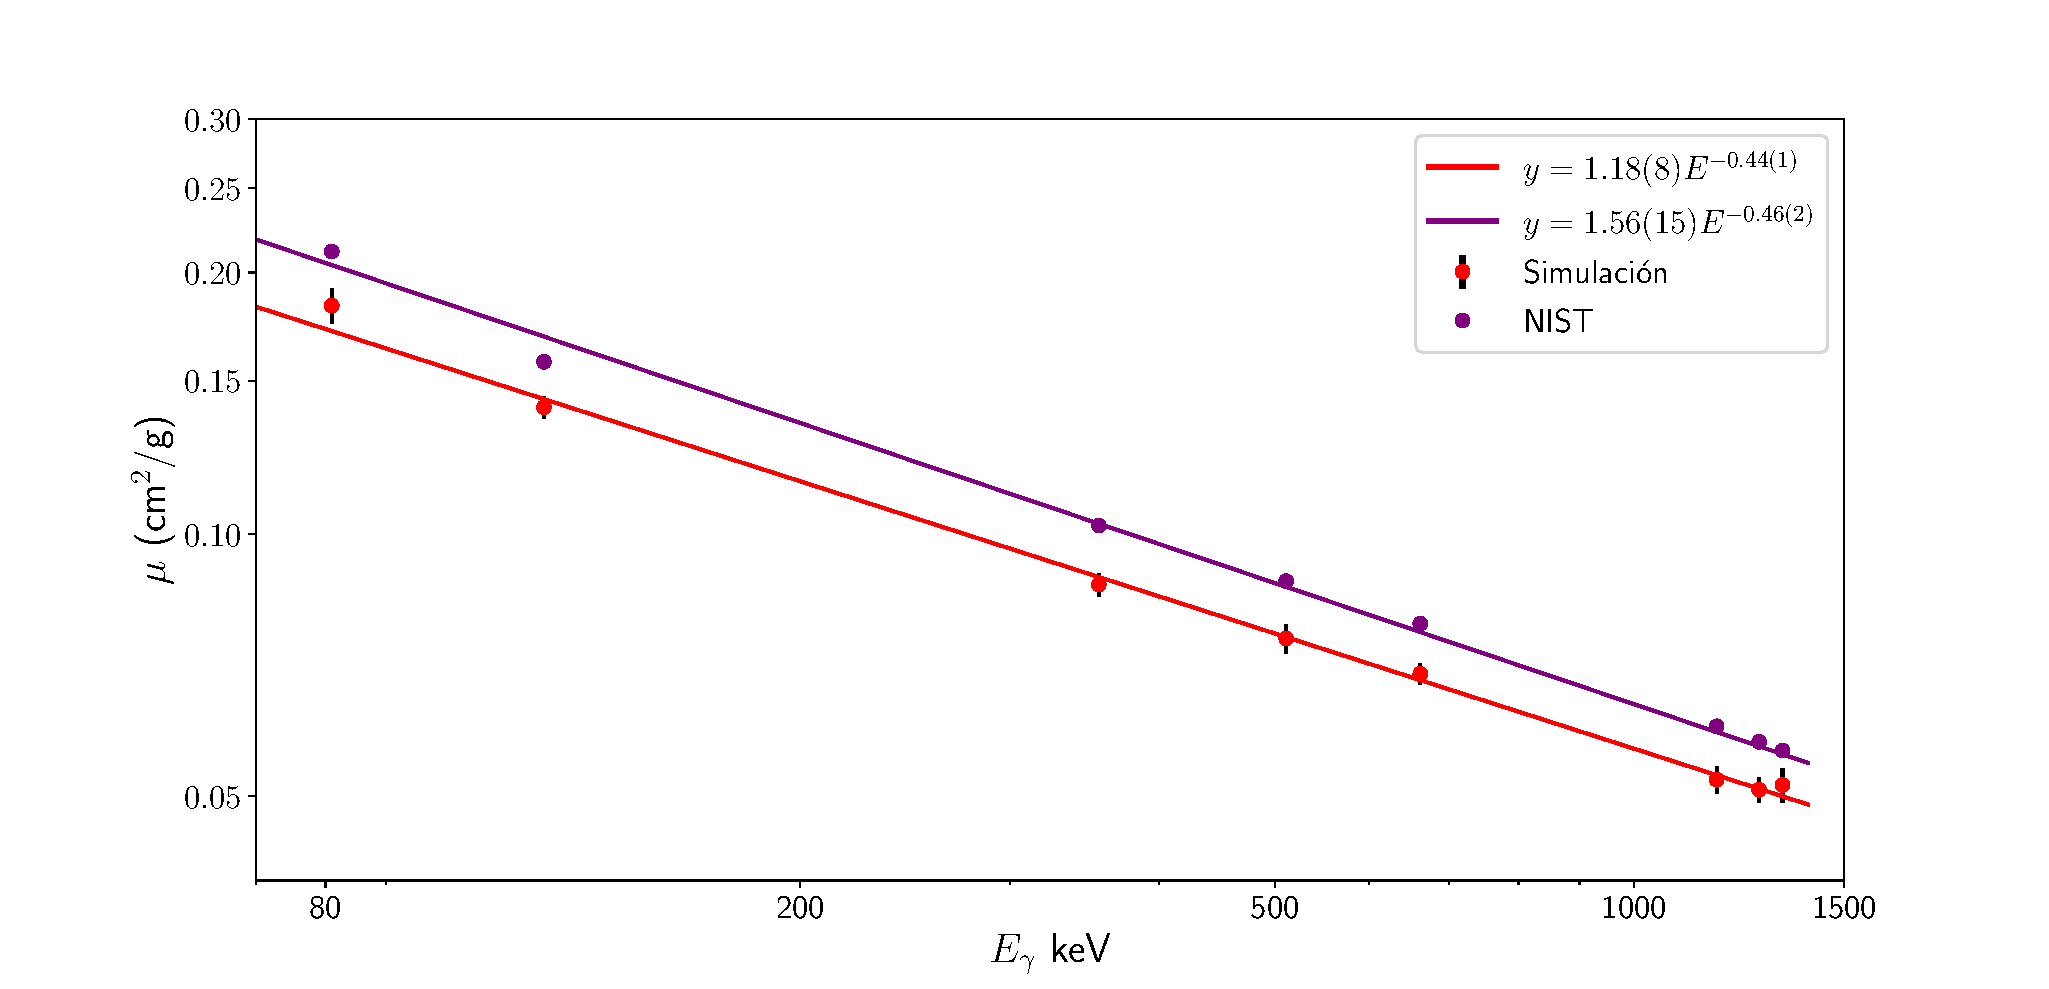
\includegraphics[width=1.0\linewidth]{Kap4/mu-trans-m1.pdf}
	\caption{Ajuste para encontrar $\alpha$ y $n$ a partir de los diferentes $\mu$/$\rho$. Morteros1.}
	\label{fig:mu-trans-m1}
\end{figure}

En la figura anterior podemos ver los valores de interés con su respectiva incertidumbre. Es importante mencionar que allí se grafica el coeficiente de atenuación másico $\mu_T$, el cual fue definido anteriormente. Como se puede observar, los resultados obtenidos con la simulación son similares a los de la base de datos NIST. Por otro lado, la incertidumbre para los datos de NIST esta asociada unicamente al ajuste.

 
\subsection{Retrodispersión.}

\begin{figure}[H]
	\centering
	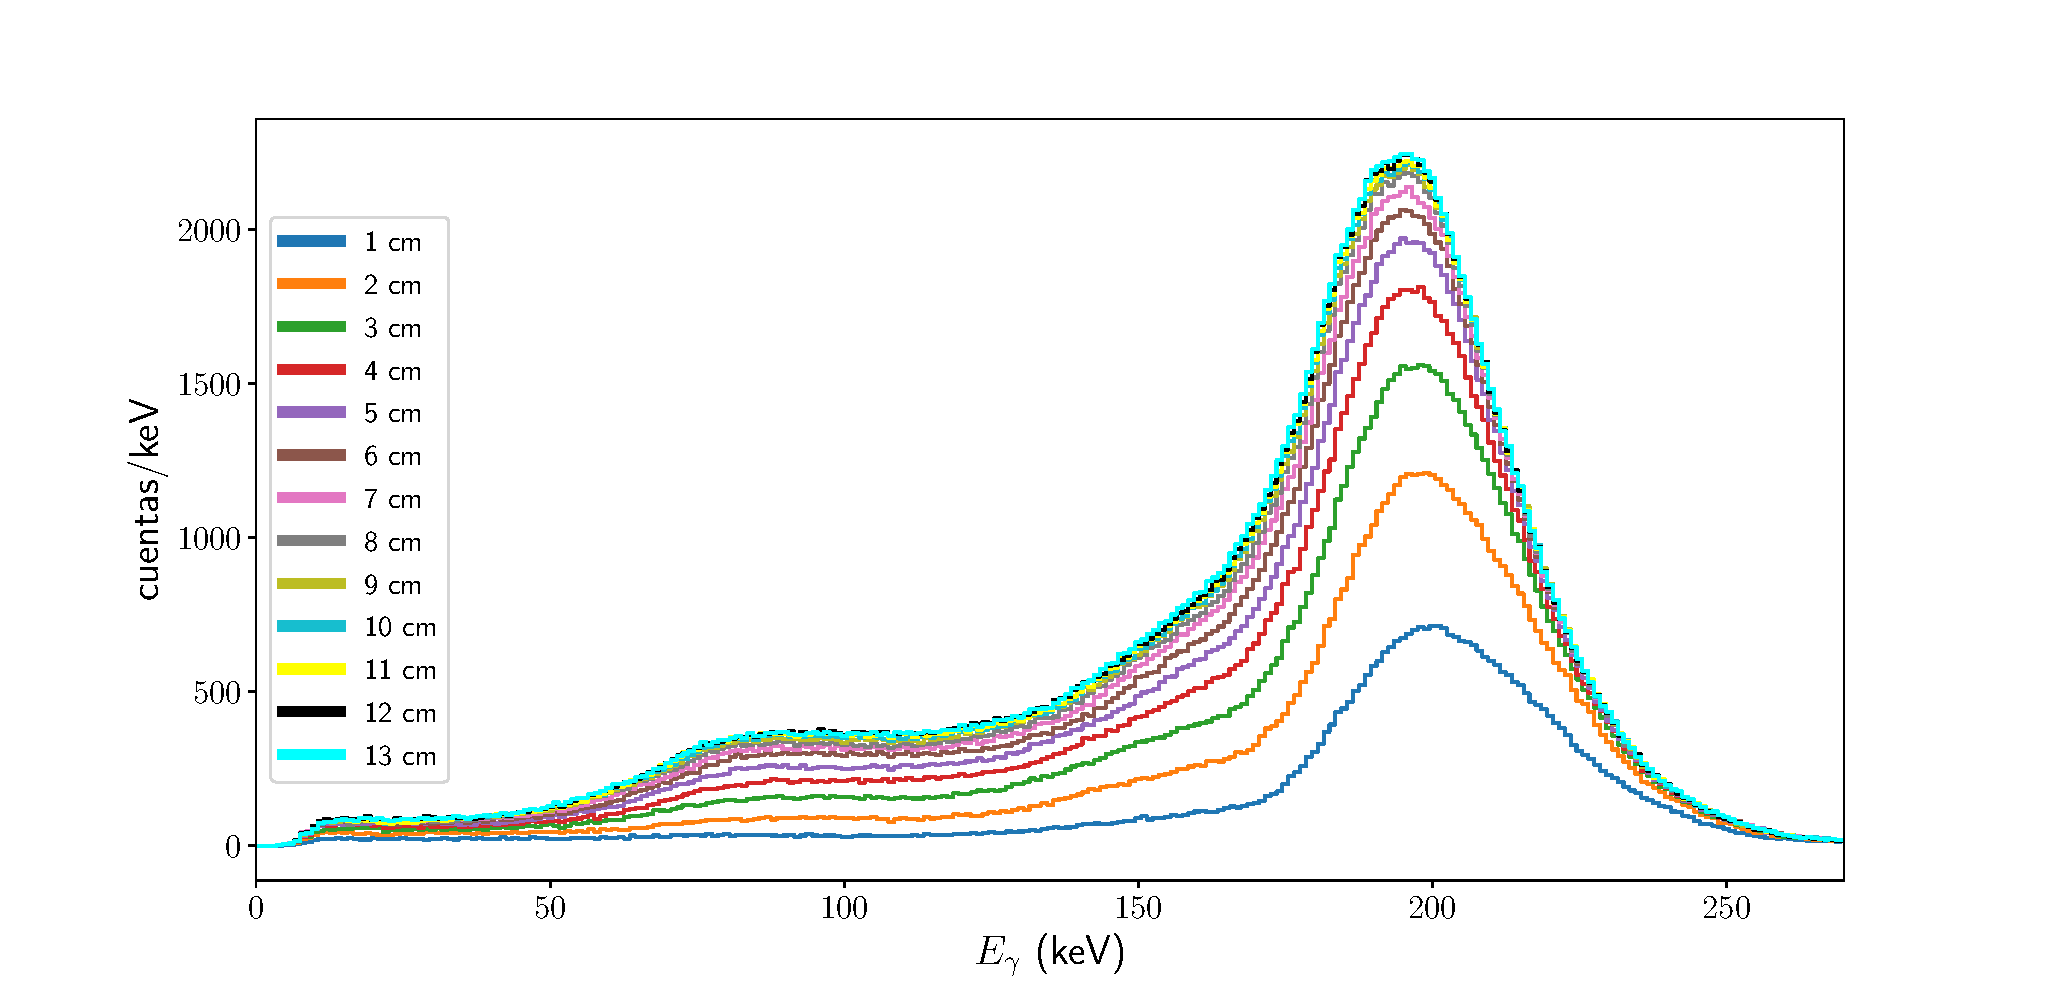
\includegraphics[width=1.0\linewidth]{Kap4/espectros_m1.pdf}
	\caption{Espectro de 10 láminas de Morteros1.}
	\label{fig:espectrosm1}
\end{figure}

En la figura \ref{fig:espectrosm1} se puede apreciar el comportamiento de las intensidades a medida que aumenta el grosor del material. De acuerdo a la figura \ref{g:Montaje-Exp-Retro} los ángulos que abarca la cara del detector mas próxima a las placas son desde $105^\circ$ hasta $164^\circ$, y las energías asociadas son $262$ keV y $197$ keV respectivamente. 
 
\begin{figure}[H]
	\centering
	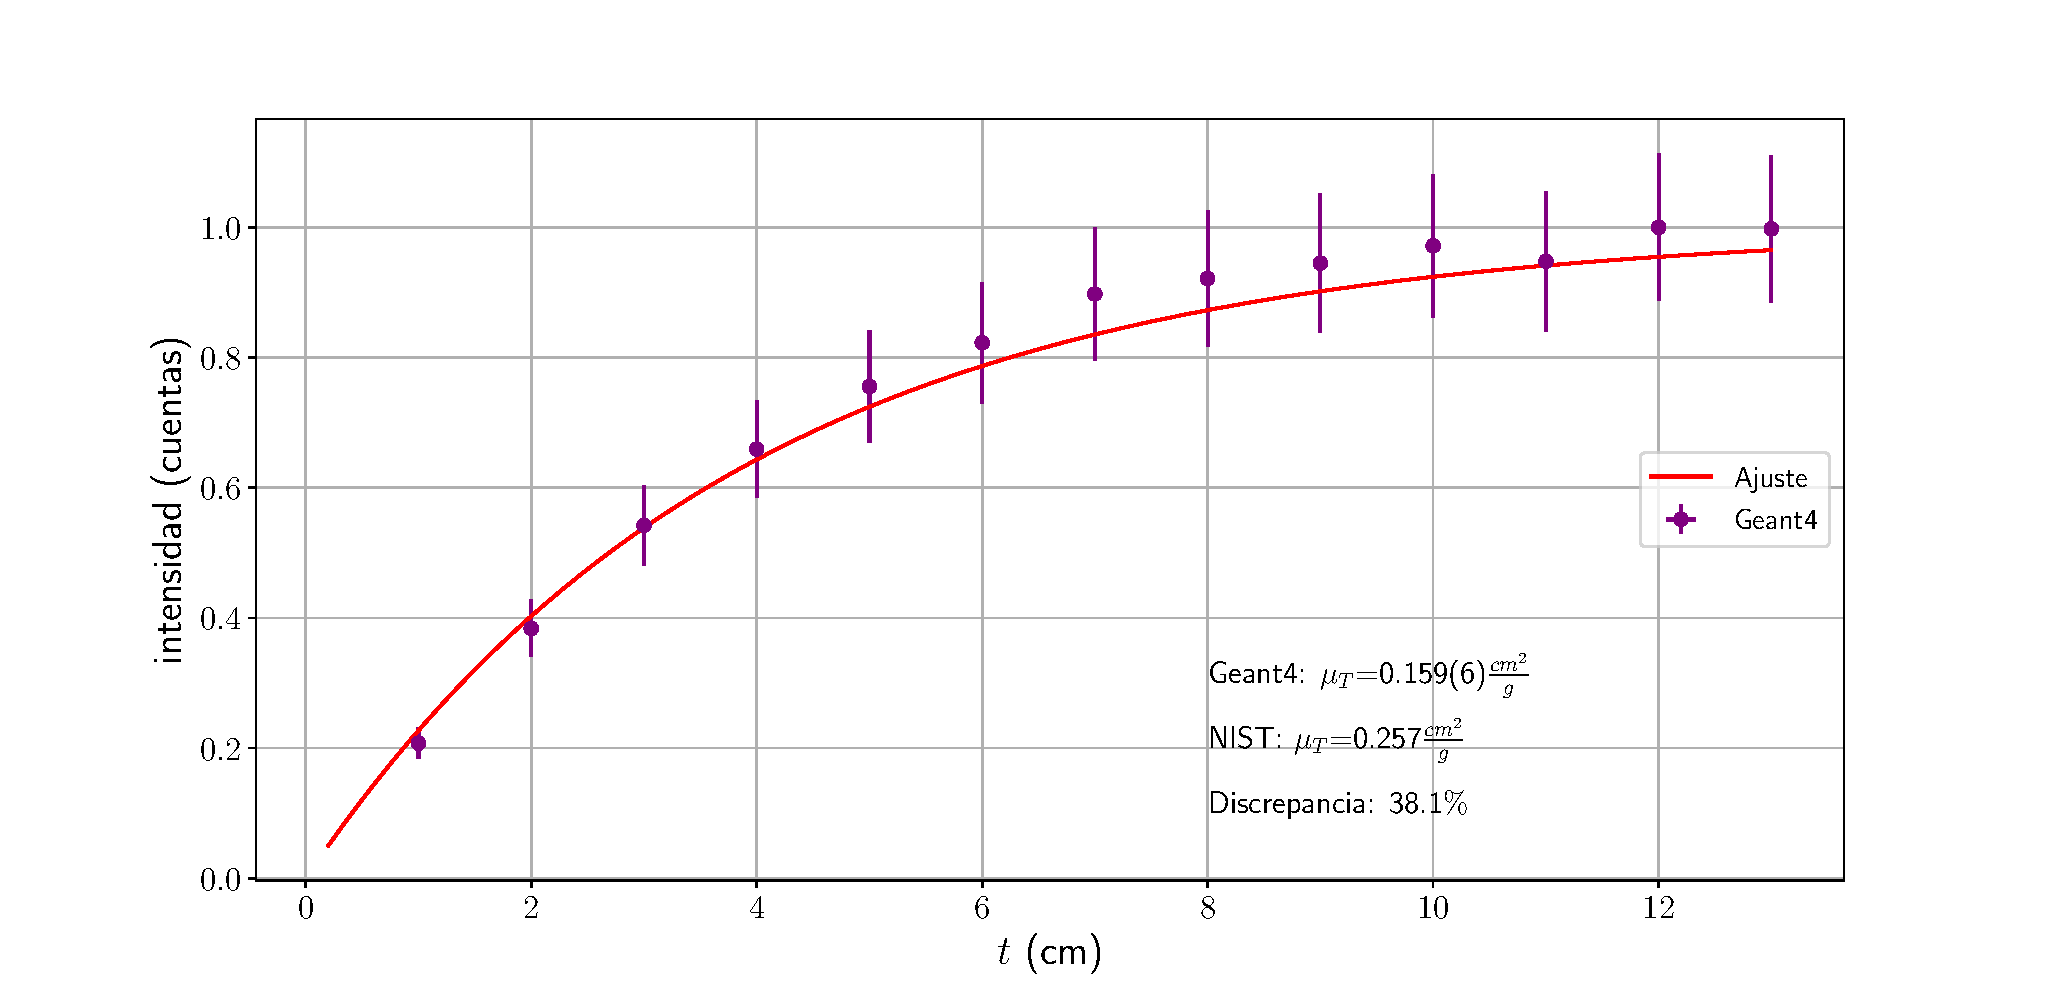
\includegraphics[width=1.0\linewidth]{Kap4/mu_T-m1.pdf}
	\caption{Valores de $\mu_T$ para Morteros 1.}
	\label{fig:mut-m1}
\end{figure}

Una vez encontradas las intensidades asociadas a cada grosor se hace un ajuste tal y como se ve en la figura \ref{fig:mut-m1}. Este ajuste permite encontrar el valor de $\mu_T$, además, de la base de datos NIST se encuentra el valor esta cantidad. Como se puede apreciar, la discrepancia entre estos dos valores es considerable.

 \section{Morteros 2.}
 
 En la tabla \ref{t:medidas-morteros2} se encuentran las dimensiones asociadas a los morteros de este lote. Es importante mencionar que dichos valores son similares con respecto al lote anterior, pues en ambos casos se usaron los mismos recipientes para la construcción.
 
 

 
 En la tabla \ref{t:materiales-mor2} se observa la composición.
 

 
 Se evidencia que la densidad no cambia mucho respecto al anterior lote, esto se debe a que la composición es similar.
 
 \begin{equation} \label{densidad-mor2}
    \rho=\frac{masa}{volumen}=1.75(5) g/cm^3
 \end{equation}
 
 \subsection{Transmisión.}
 
\begin{figure}[H]
	\centering
	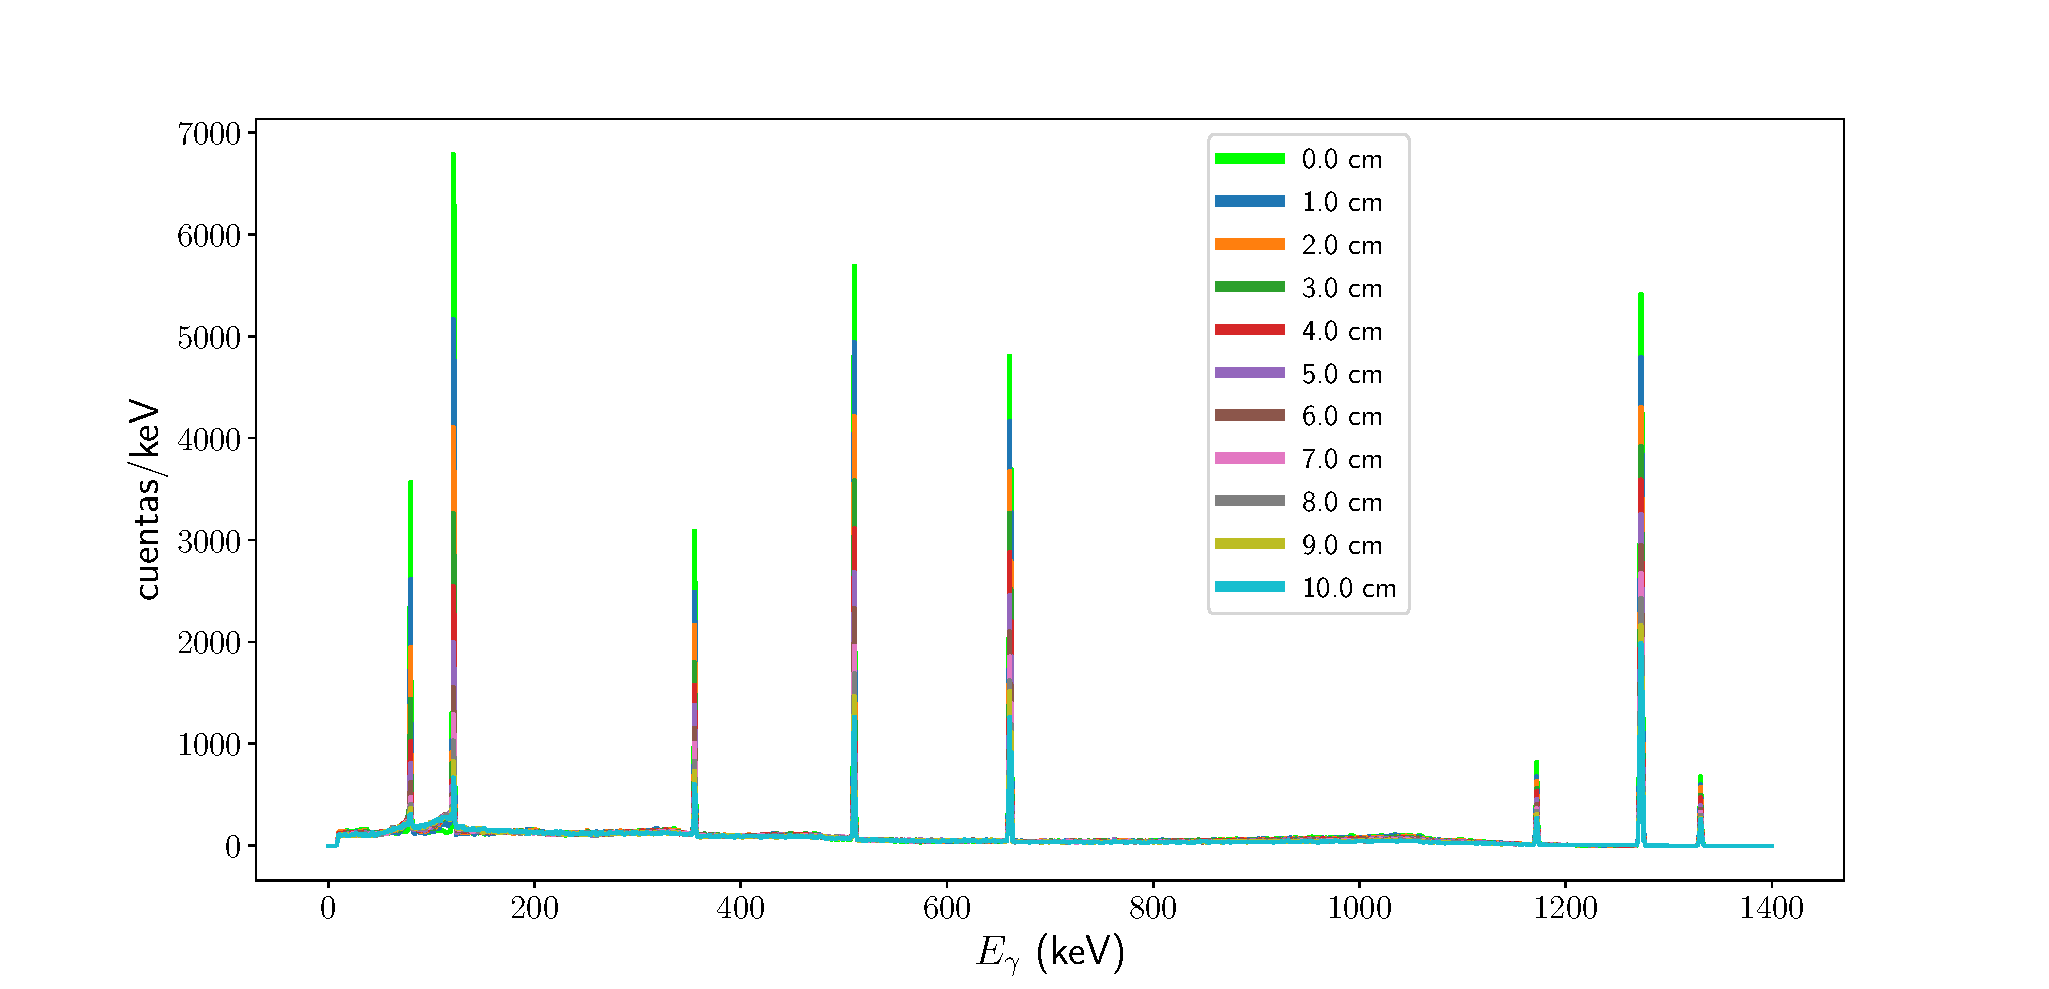
\includegraphics[width=1.0\linewidth]{Kap4/espectro_m2-10M-trans.pdf}
	\caption{Espectro de 10 láminas de Morteros2. Transmisión.}
	\label{fig:espectrom2-10m-trans}
\end{figure}
 
 
\begin{figure}[H]
	\centering
	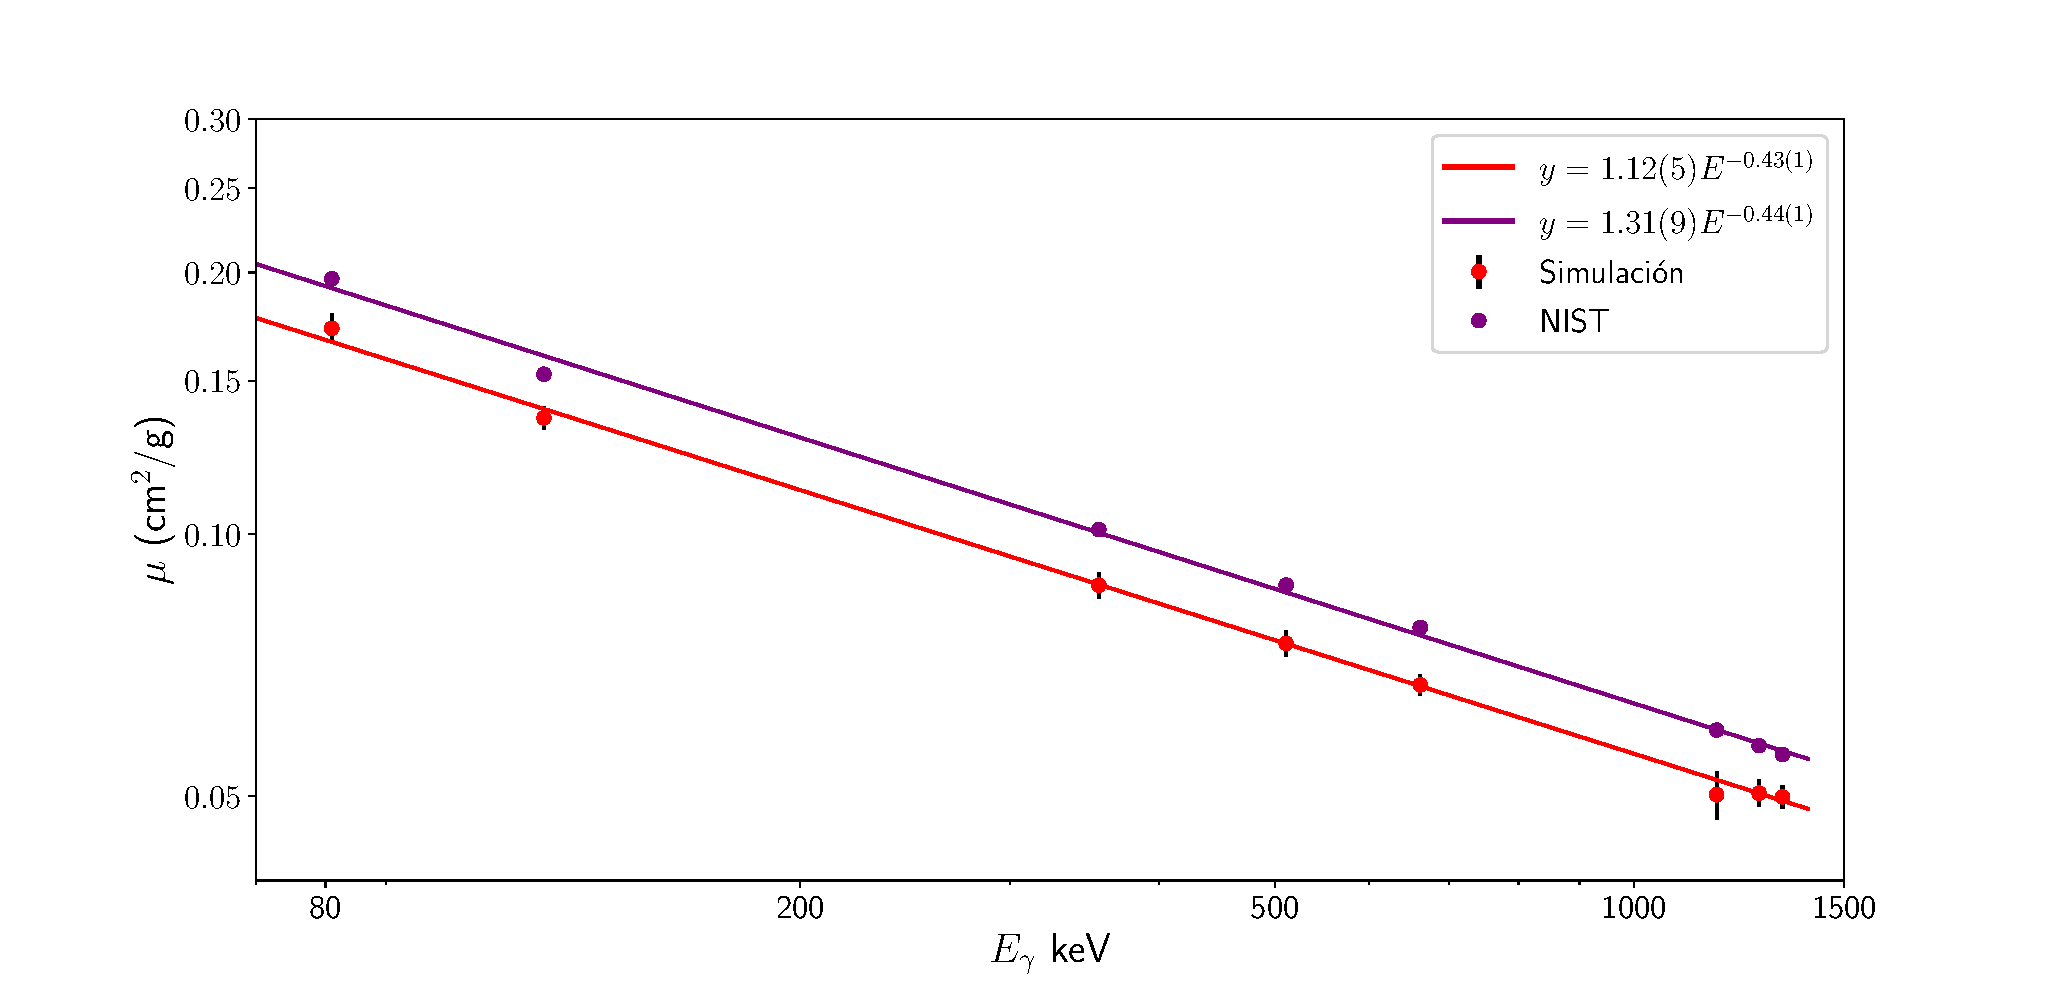
\includegraphics[width=1.0\linewidth]{Kap4/mu-trans-m2.pdf}
	\caption{Ajuste para encontrar $\alpha$ y $n$ a partir de los diferentes $\mu$/$\rho$. Morteros2.}
	\label{fig:mu-trans-m2}
\end{figure}
 
 
 \subsection{Retrodispersión.}
 
 
\begin{figure}[H]
	\centering
	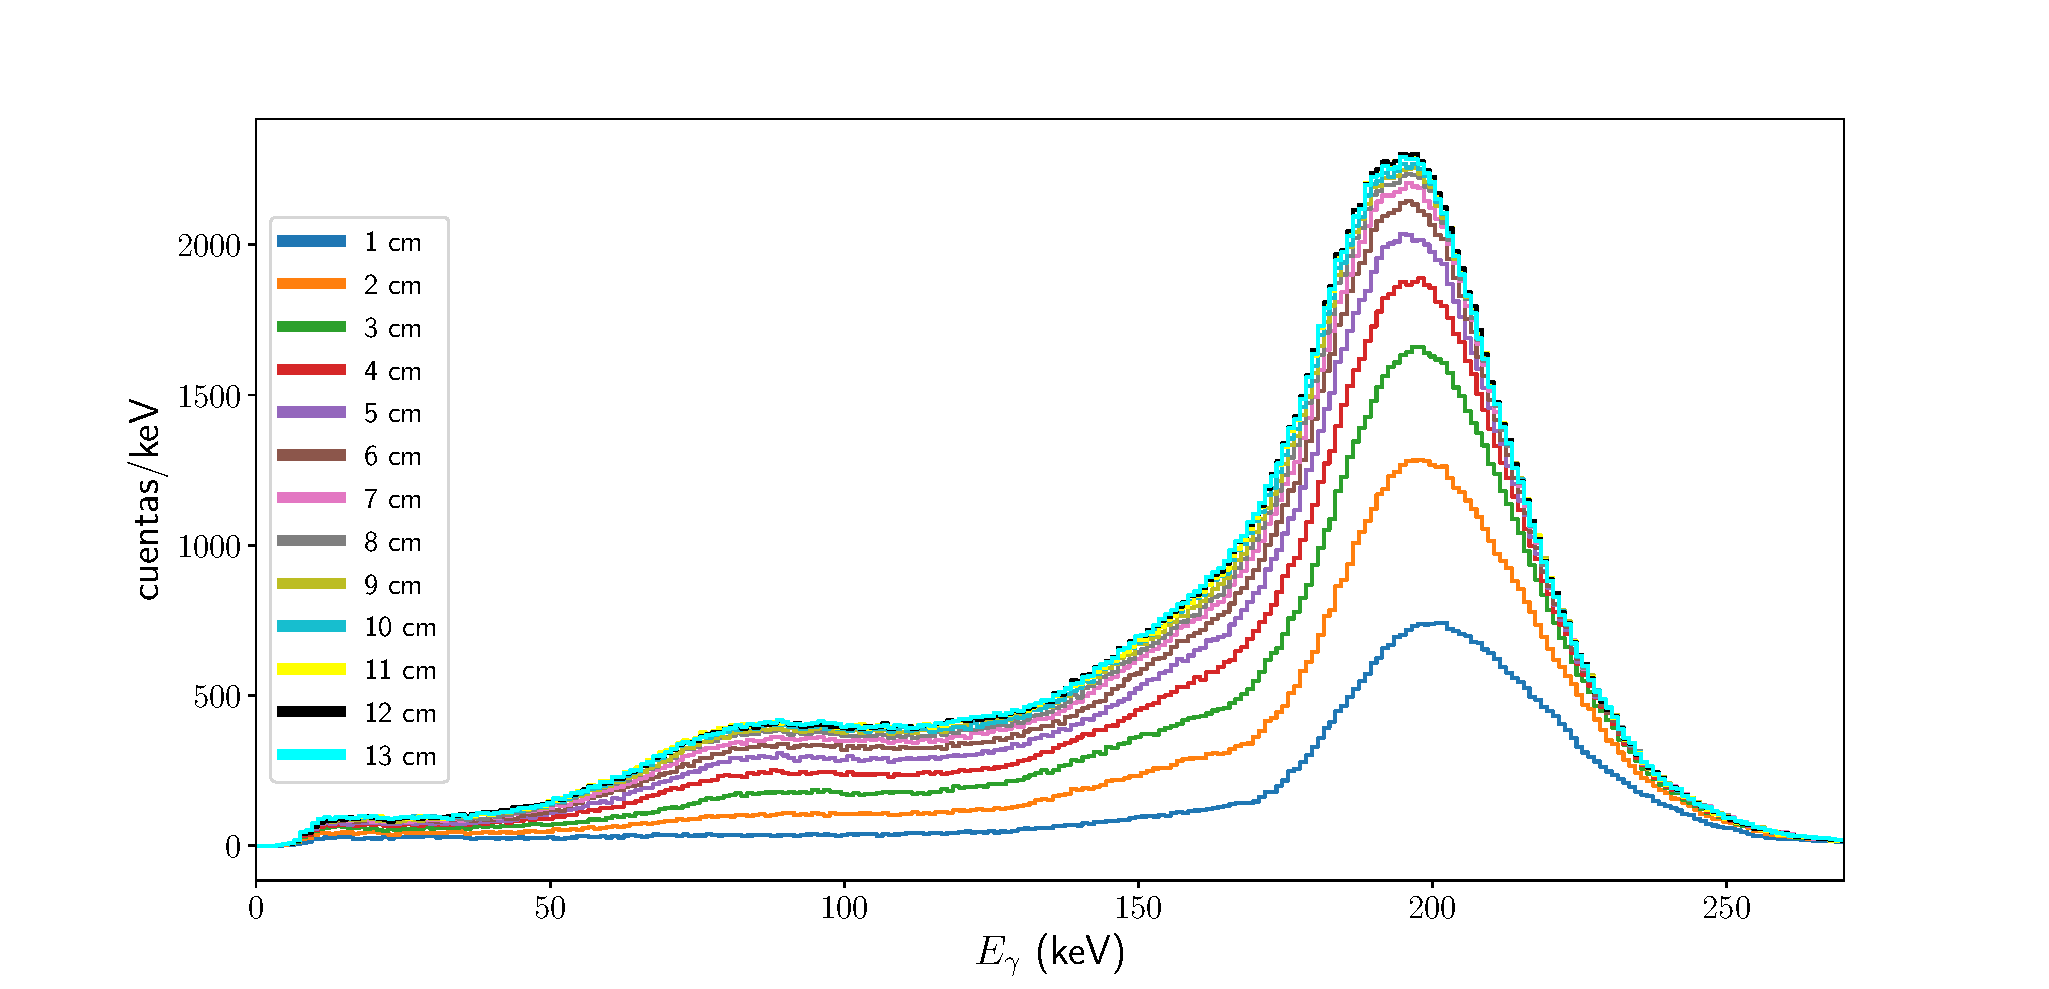
\includegraphics[width=1.0\linewidth]{Kap4/espectro_m2.pdf}
	\caption{Espectro de 10 láminas de Morteros1.}
	\label{fig:espectrom2}
\end{figure}
 
\begin{figure}[H]
	\centering
	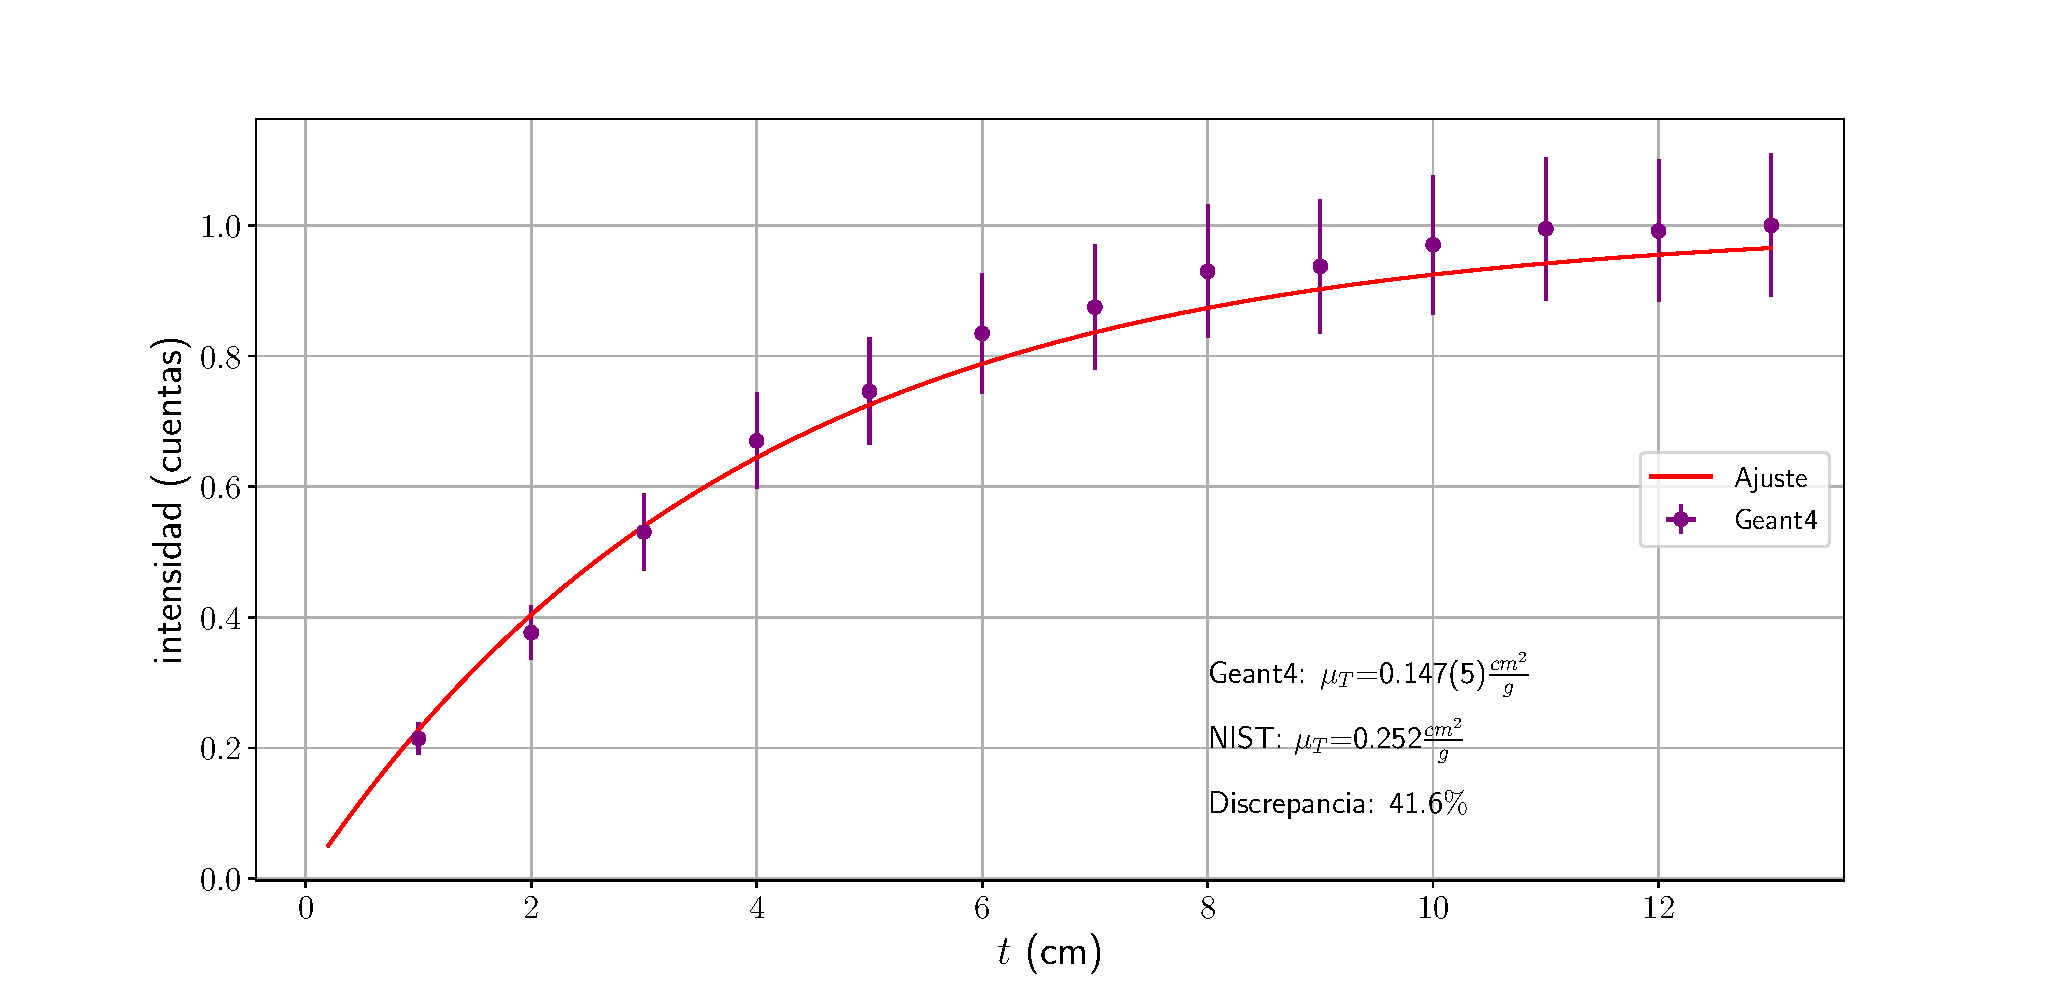
\includegraphics[width=1.0\linewidth]{Kap4/mu_T-m2.pdf}
	\caption{Valores para $\mu_T$. Morteros2.}
	\label{fig:mut-m2}
\end{figure}
 
 
 
 \section{Morteros 3.}
 

 
 

 
 \begin{equation} \label{densidad-mor3}
 \rho=\frac{masa}{volumen}=1.62(7) g/cm^3
 \end{equation}
 
 \subsection{Transmisión.}
 
\begin{figure}[H]
	\centering
	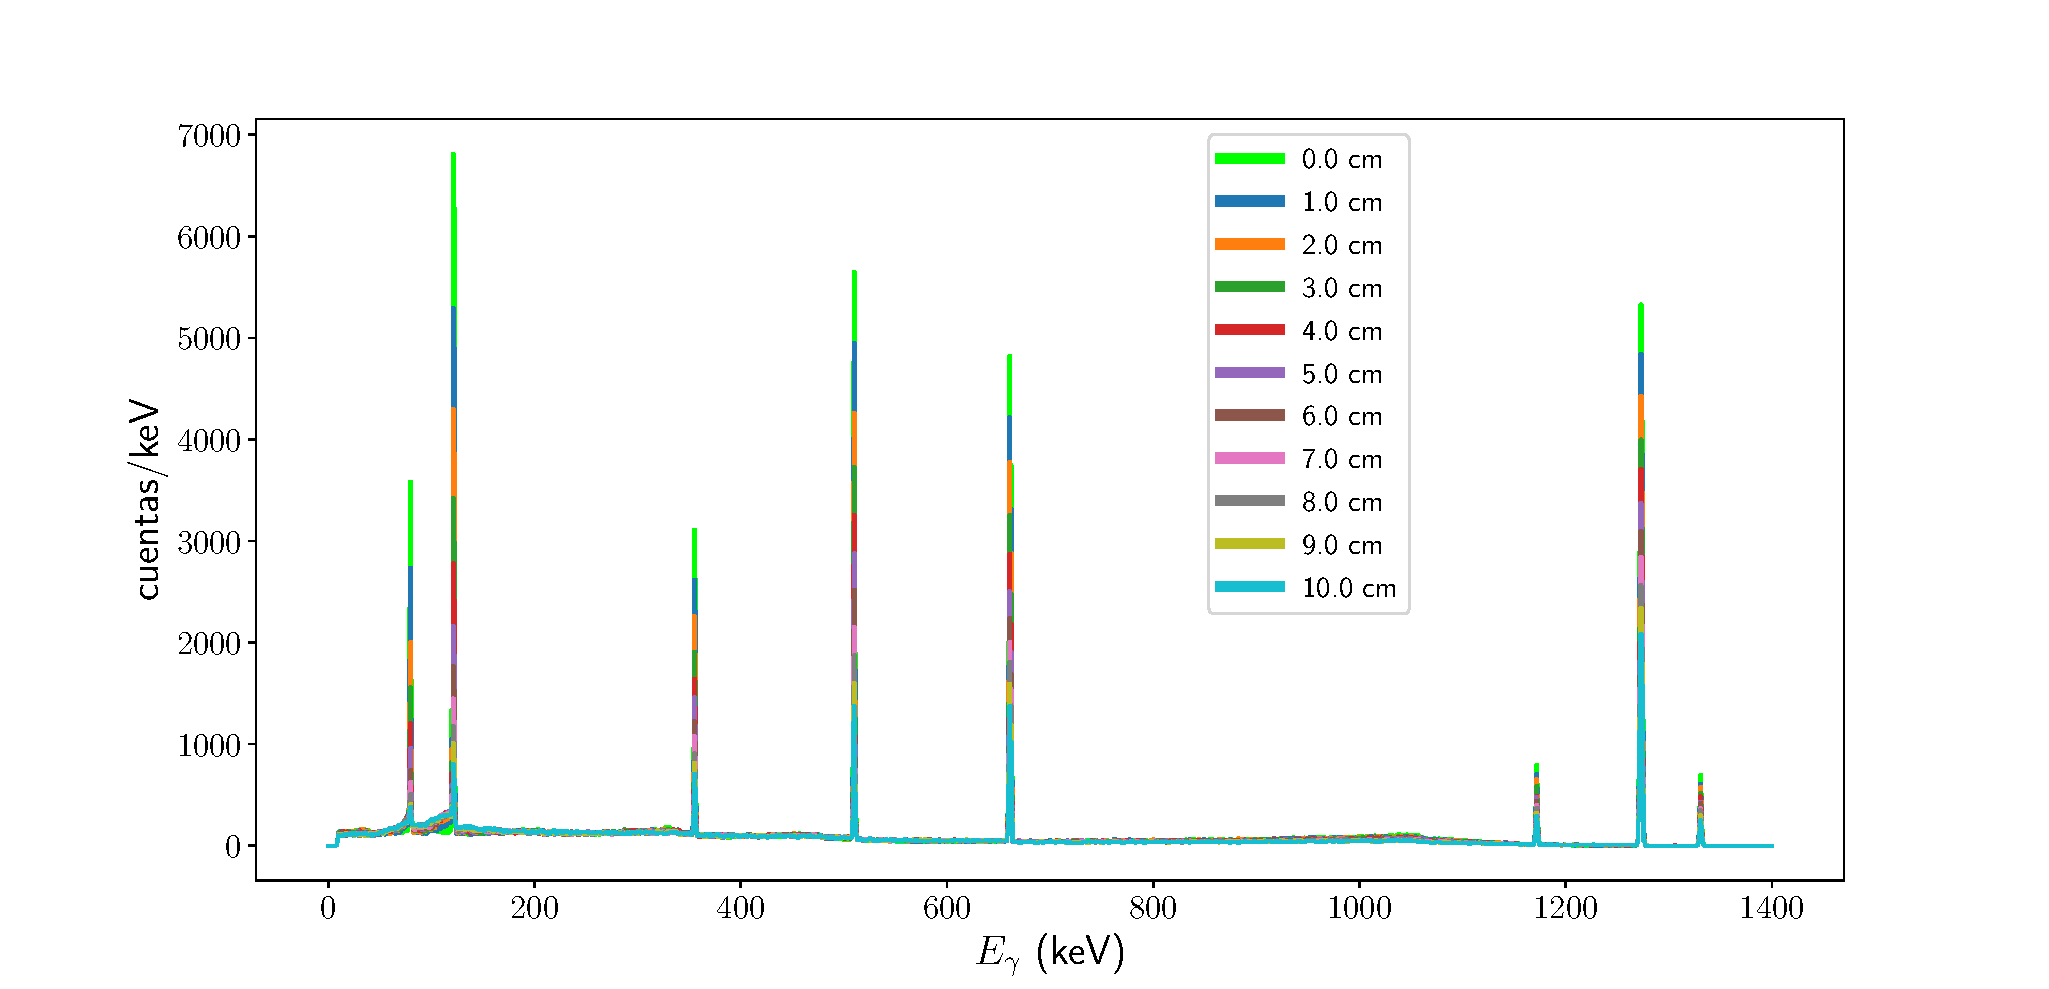
\includegraphics[width=1.0\linewidth]{Kap4/espectro_m3-M10-trans.pdf}
	\caption{Espectro de 10 láminas de Morteros3. Transmisión}
	\label{fig:espectrom3-m10-trans}
\end{figure}
 
\begin{figure}[H]
	\centering
	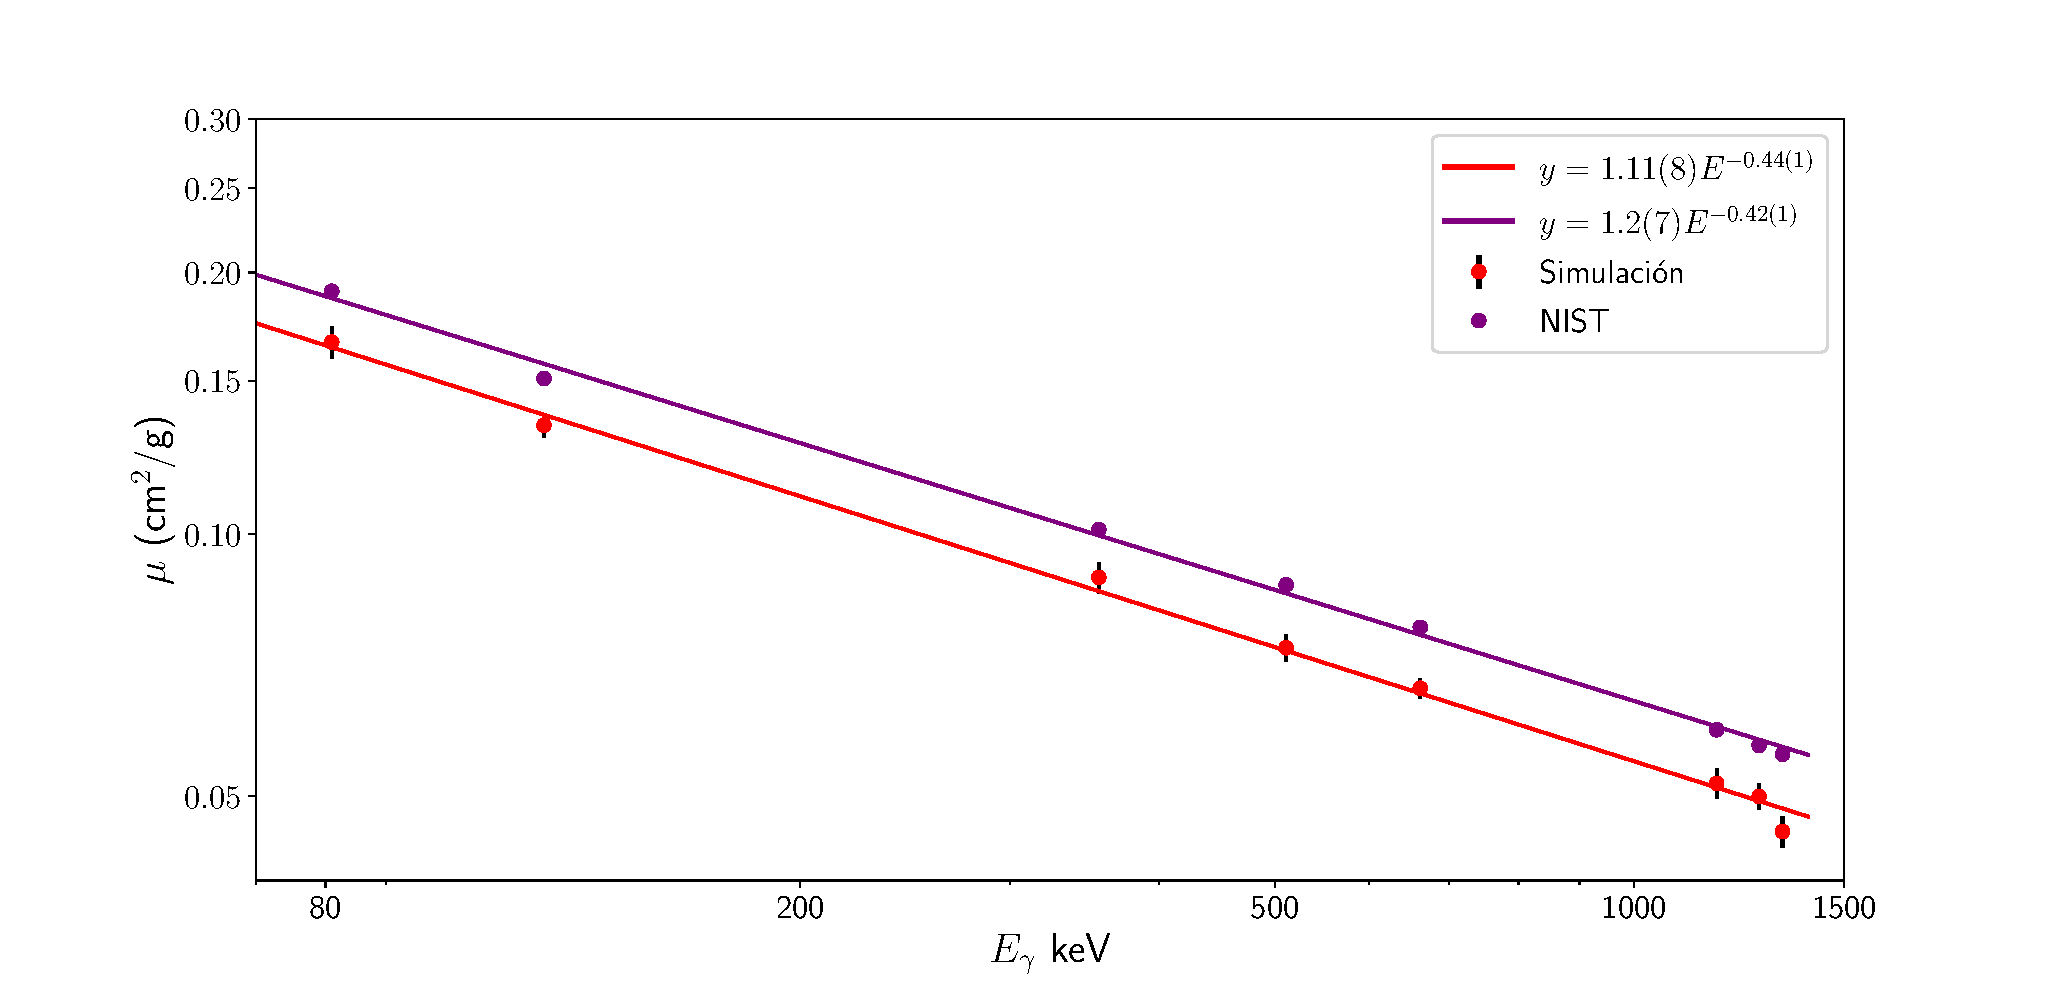
\includegraphics[width=1.0\linewidth]{Kap4/mu-trans-m3.pdf}
	\caption{Ajuste para encontrar $\alpha$ y $n$ a partir de los diferentes $\mu$/$\rho$. Morteros3.}
	\label{fig:mu-trans-m3}
\end{figure}
 
 
 \subsection{Retrodispersión.}
 
\begin{figure}[H]
	\centering
	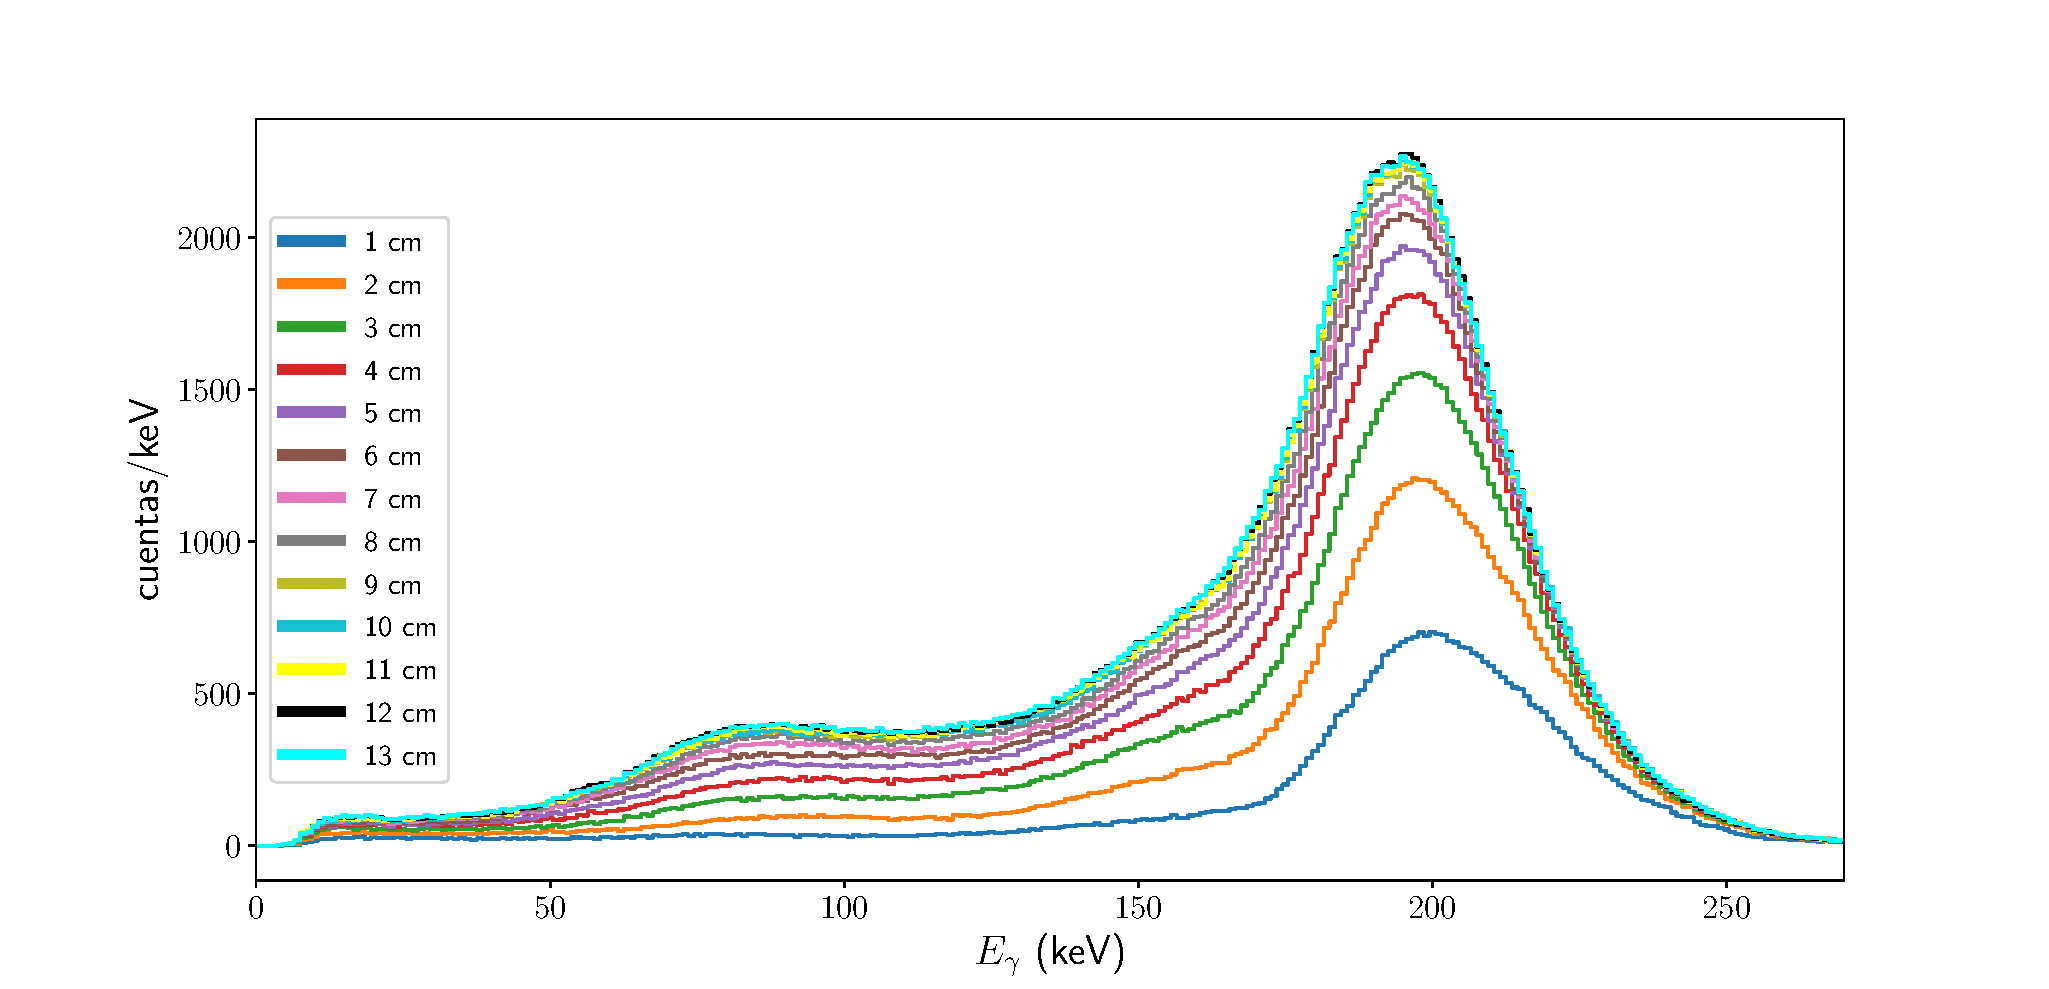
\includegraphics[width=1.0\linewidth]{Kap4/espectro_m3.pdf}
	\caption{Espectro de 10 láminas de Morteros3.}
	\label{fig:espectrom3}
\end{figure}

\begin{figure}[H]
	\centering
	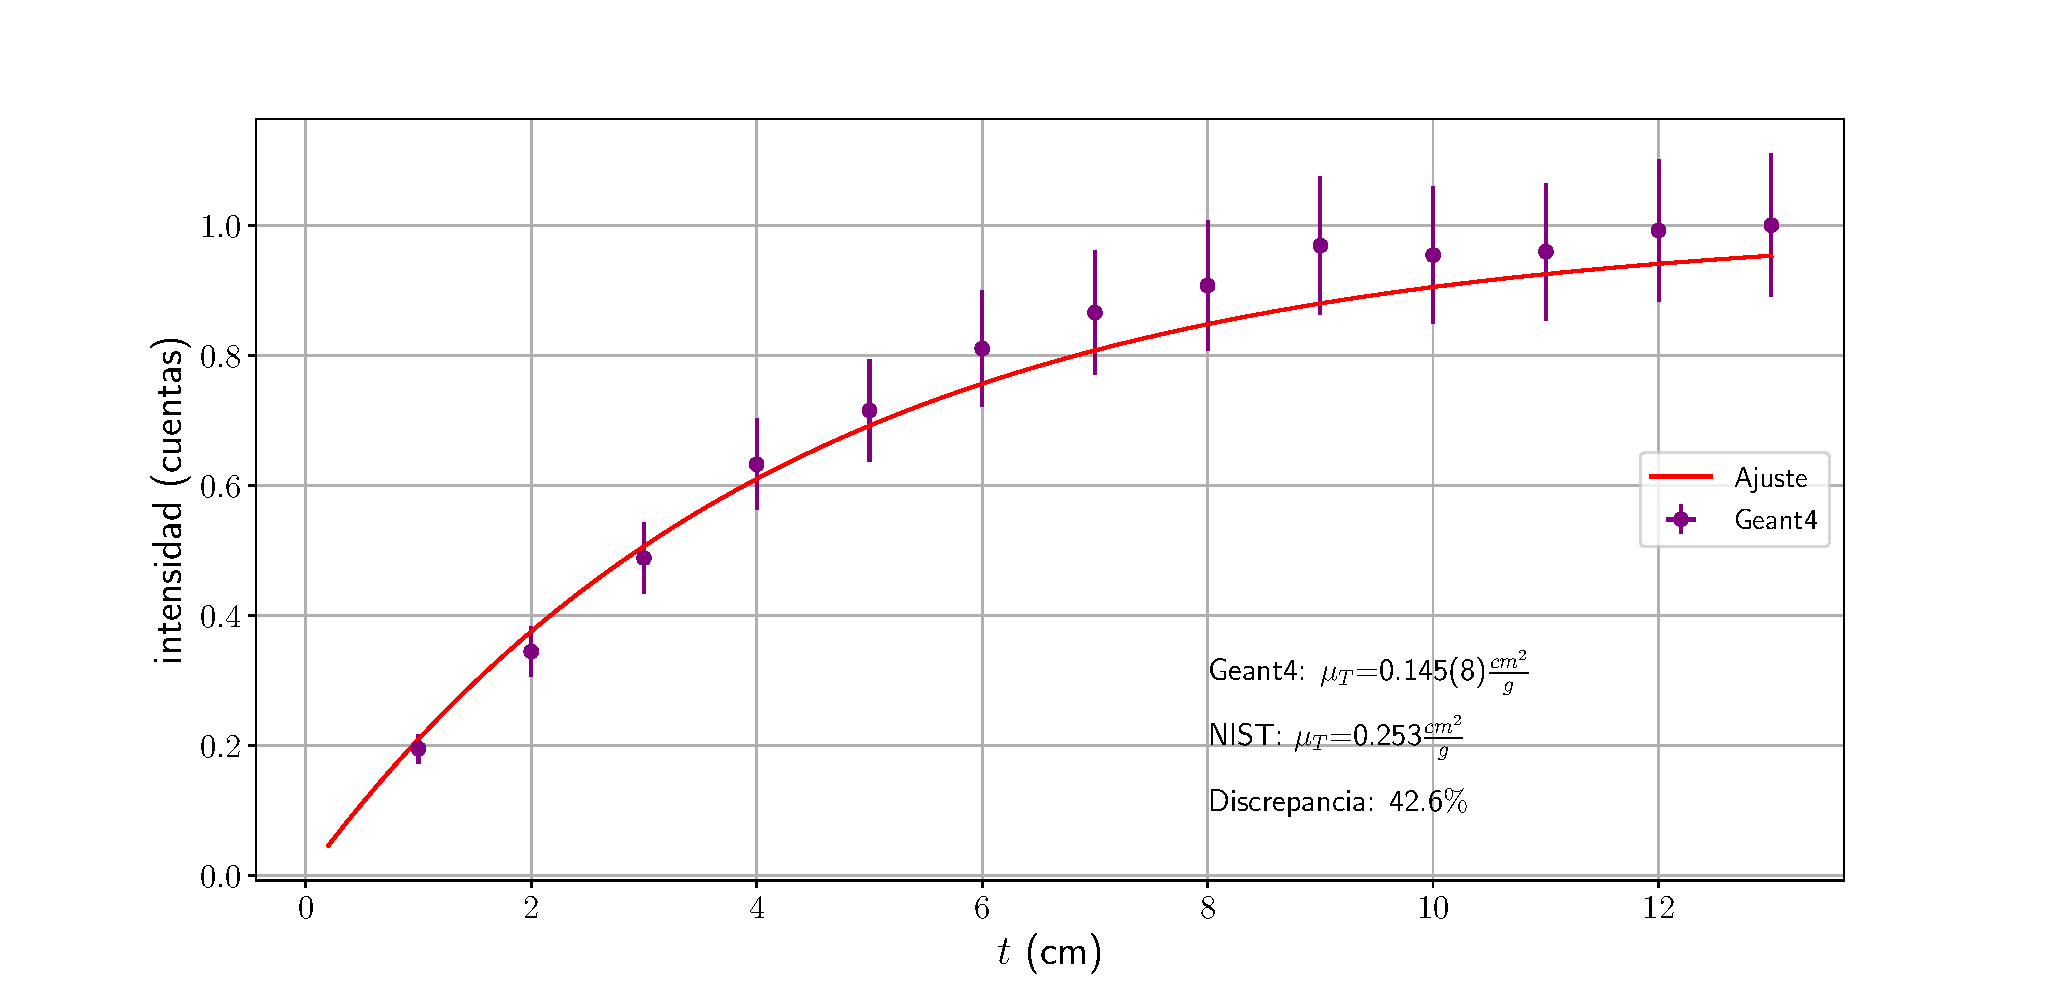
\includegraphics[width=1.0\linewidth]{Kap4/mu_T-m3.pdf}
	\caption{$\mu_T=0.24(1) cm^{-1}$ Morteros3.}
	\label{fig:mut-m3}
\end{figure}

 
 
 
 \section{Morteros 4.}
 


 
 \begin{equation} \label{densidad-mor4}
 \rho=\frac{masa}{volumen}=1.62(3) g/cm^3
 \end{equation}
 
 \subsection{Transmisión.}
 
\begin{figure}[H]
	\centering
	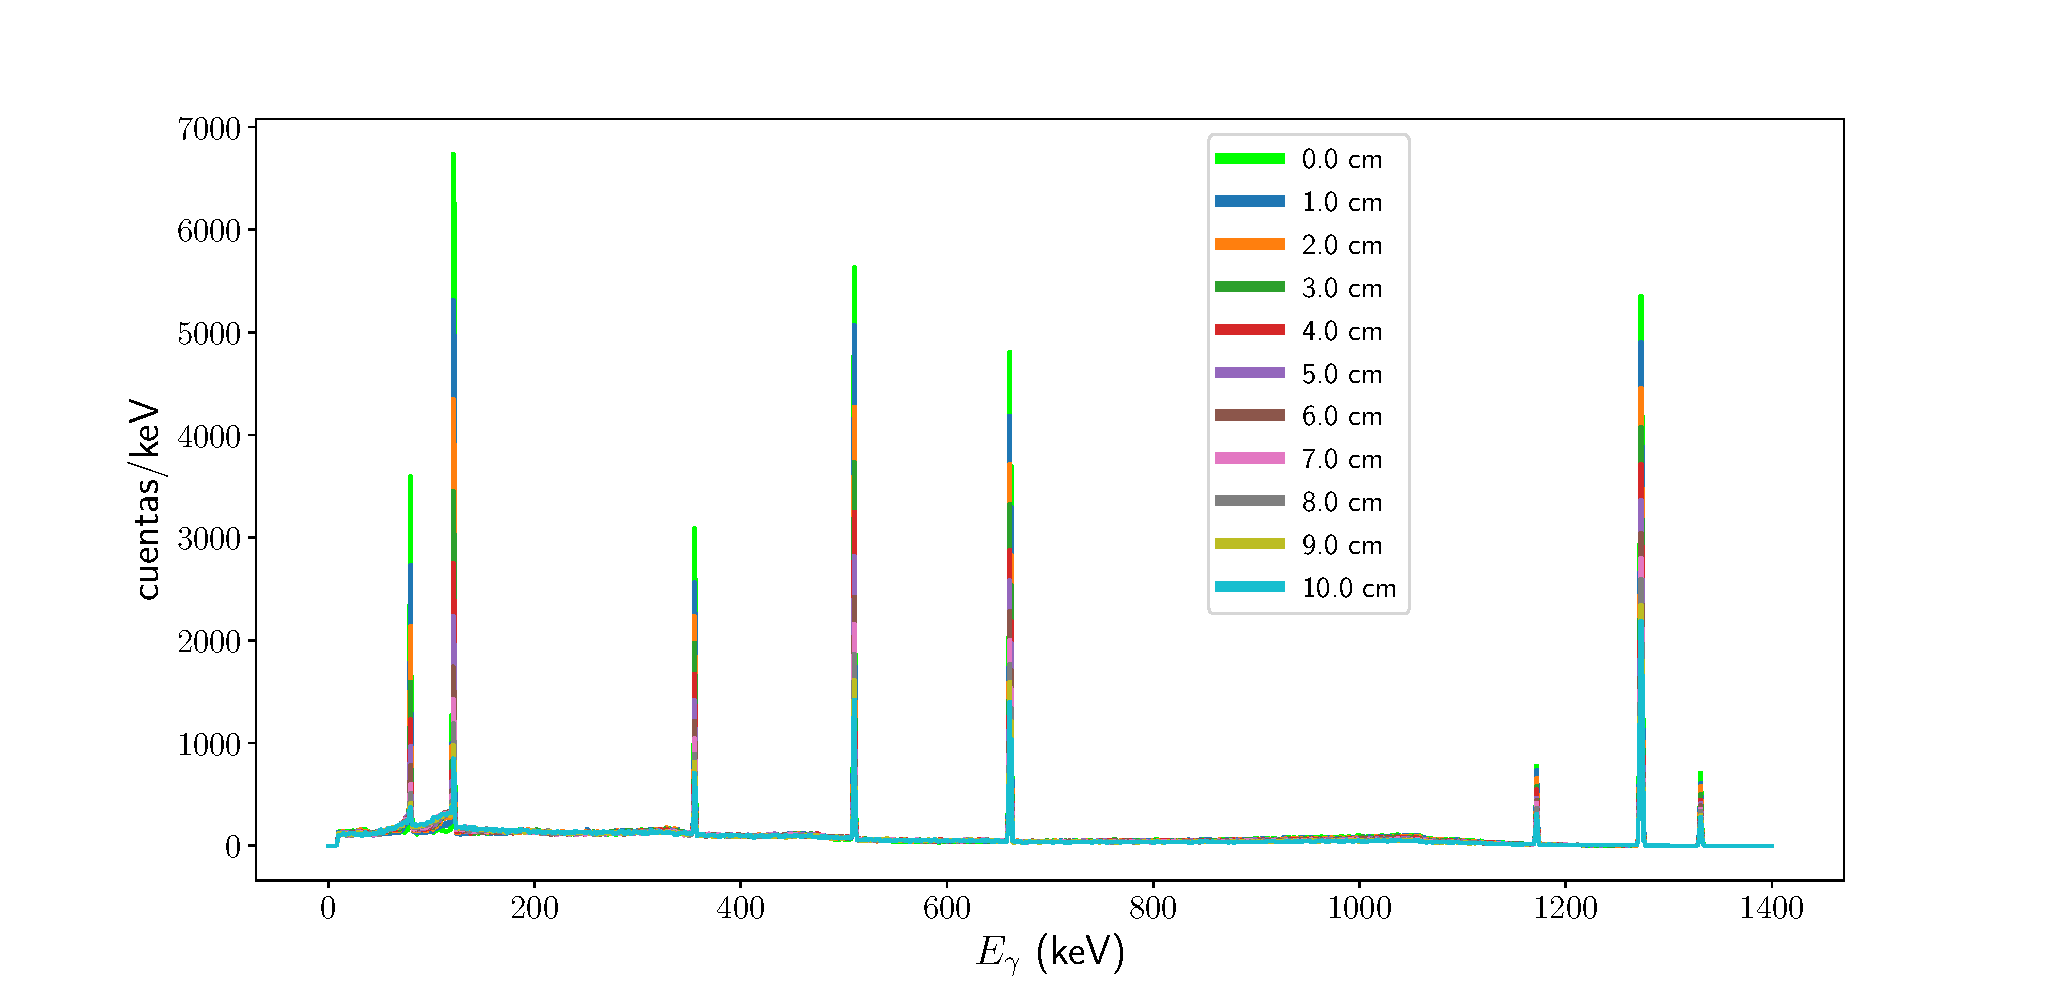
\includegraphics[width=1.0\linewidth]{Kap4/espectro_m4-10M-trans.pdf}
	\caption{Espectro de 10 láminas de Morteros4. Transmisicón}
	\label{fig:espectrom4-10m-trans}
\end{figure}
 
\begin{figure}[H]
	\centering
	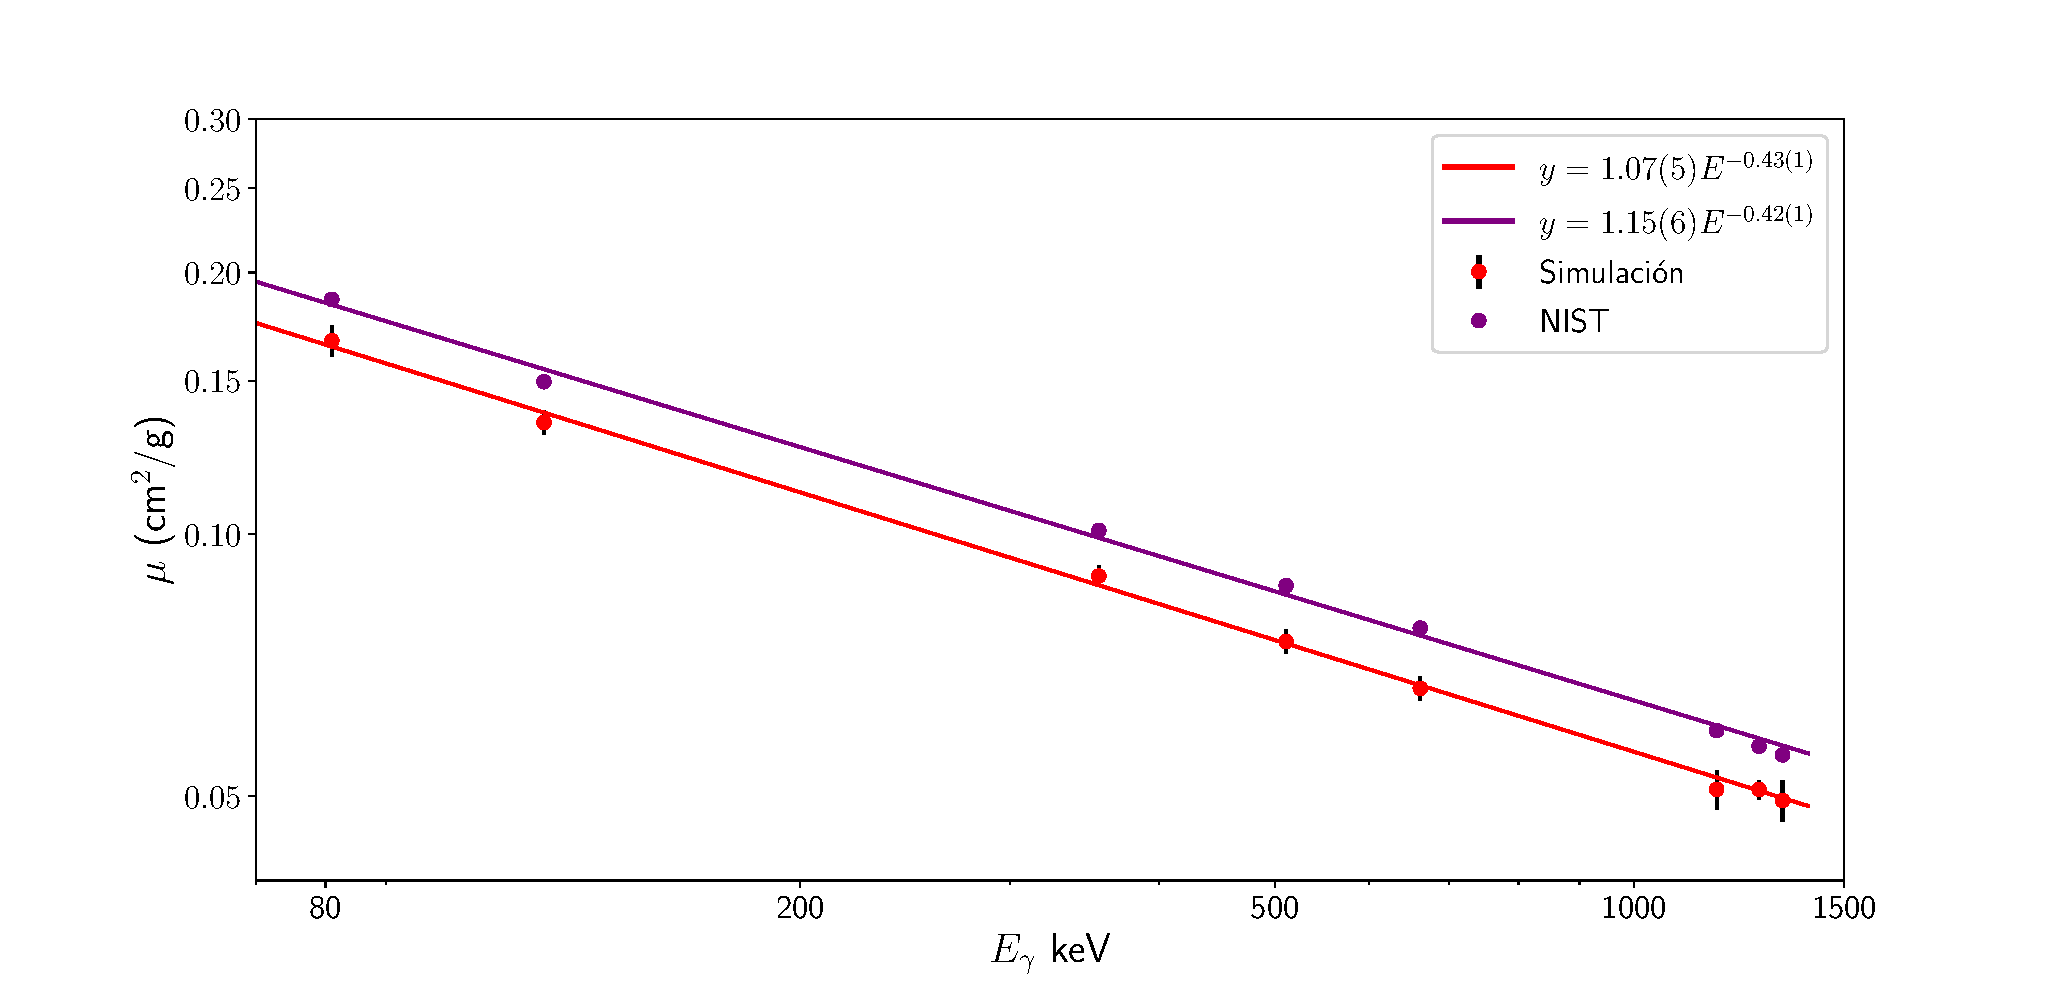
\includegraphics[width=1.0\linewidth]{Kap4/mu-trans-m4.pdf}
	\caption{Ajuste para encontrar $\alpha$ y $n$ a partir de los diferentes $\mu$/$\rho$. Morteros4.}
	\label{fig:mu-trans-m4}
\end{figure}
 
 
 \subsection{Retrodispersión.}
 
 \begin{figure}[H]
 	\centering
 	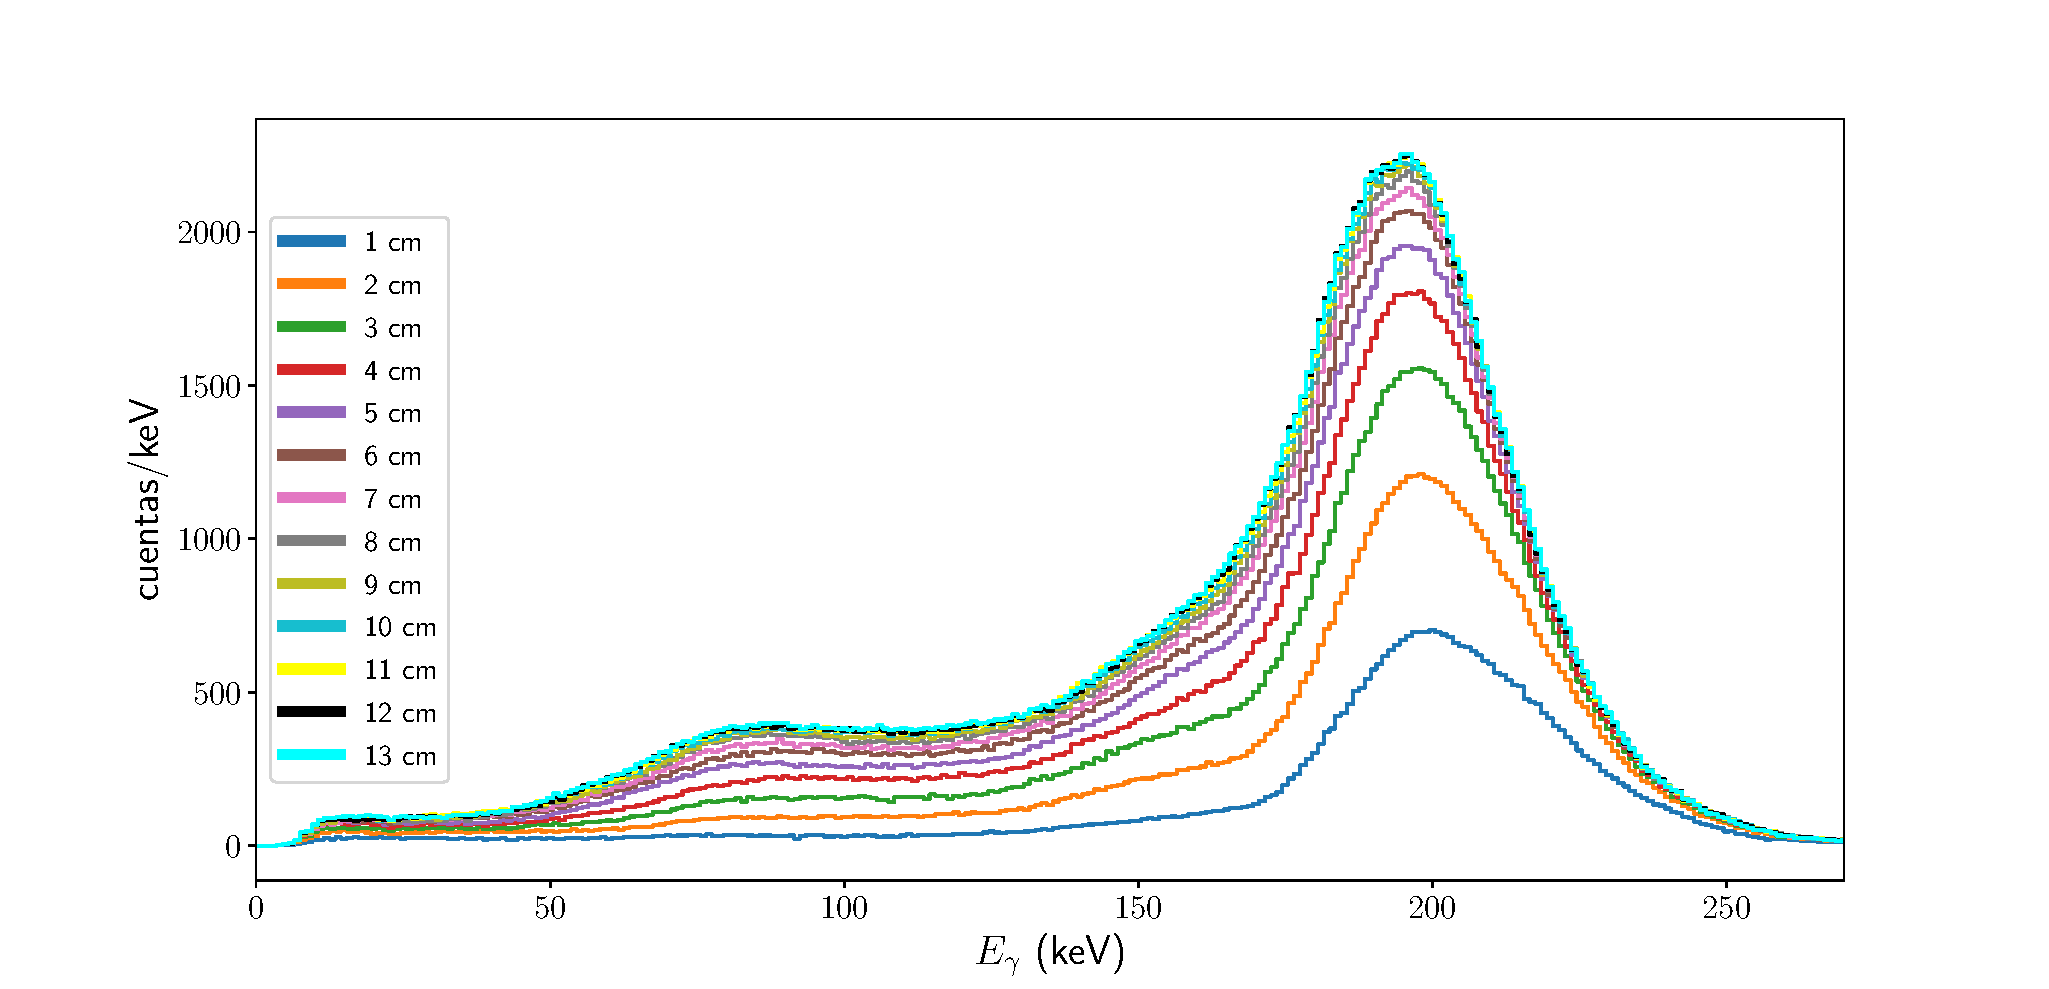
\includegraphics[width=1.0\linewidth]{Kap4/espectro_m4.pdf}
 	\caption{Espectro de 10 láminas de Morteros4.}
 	\label{fig:espectrom4}
 \end{figure}
 
 \begin{figure}[H]
 	\centering
 	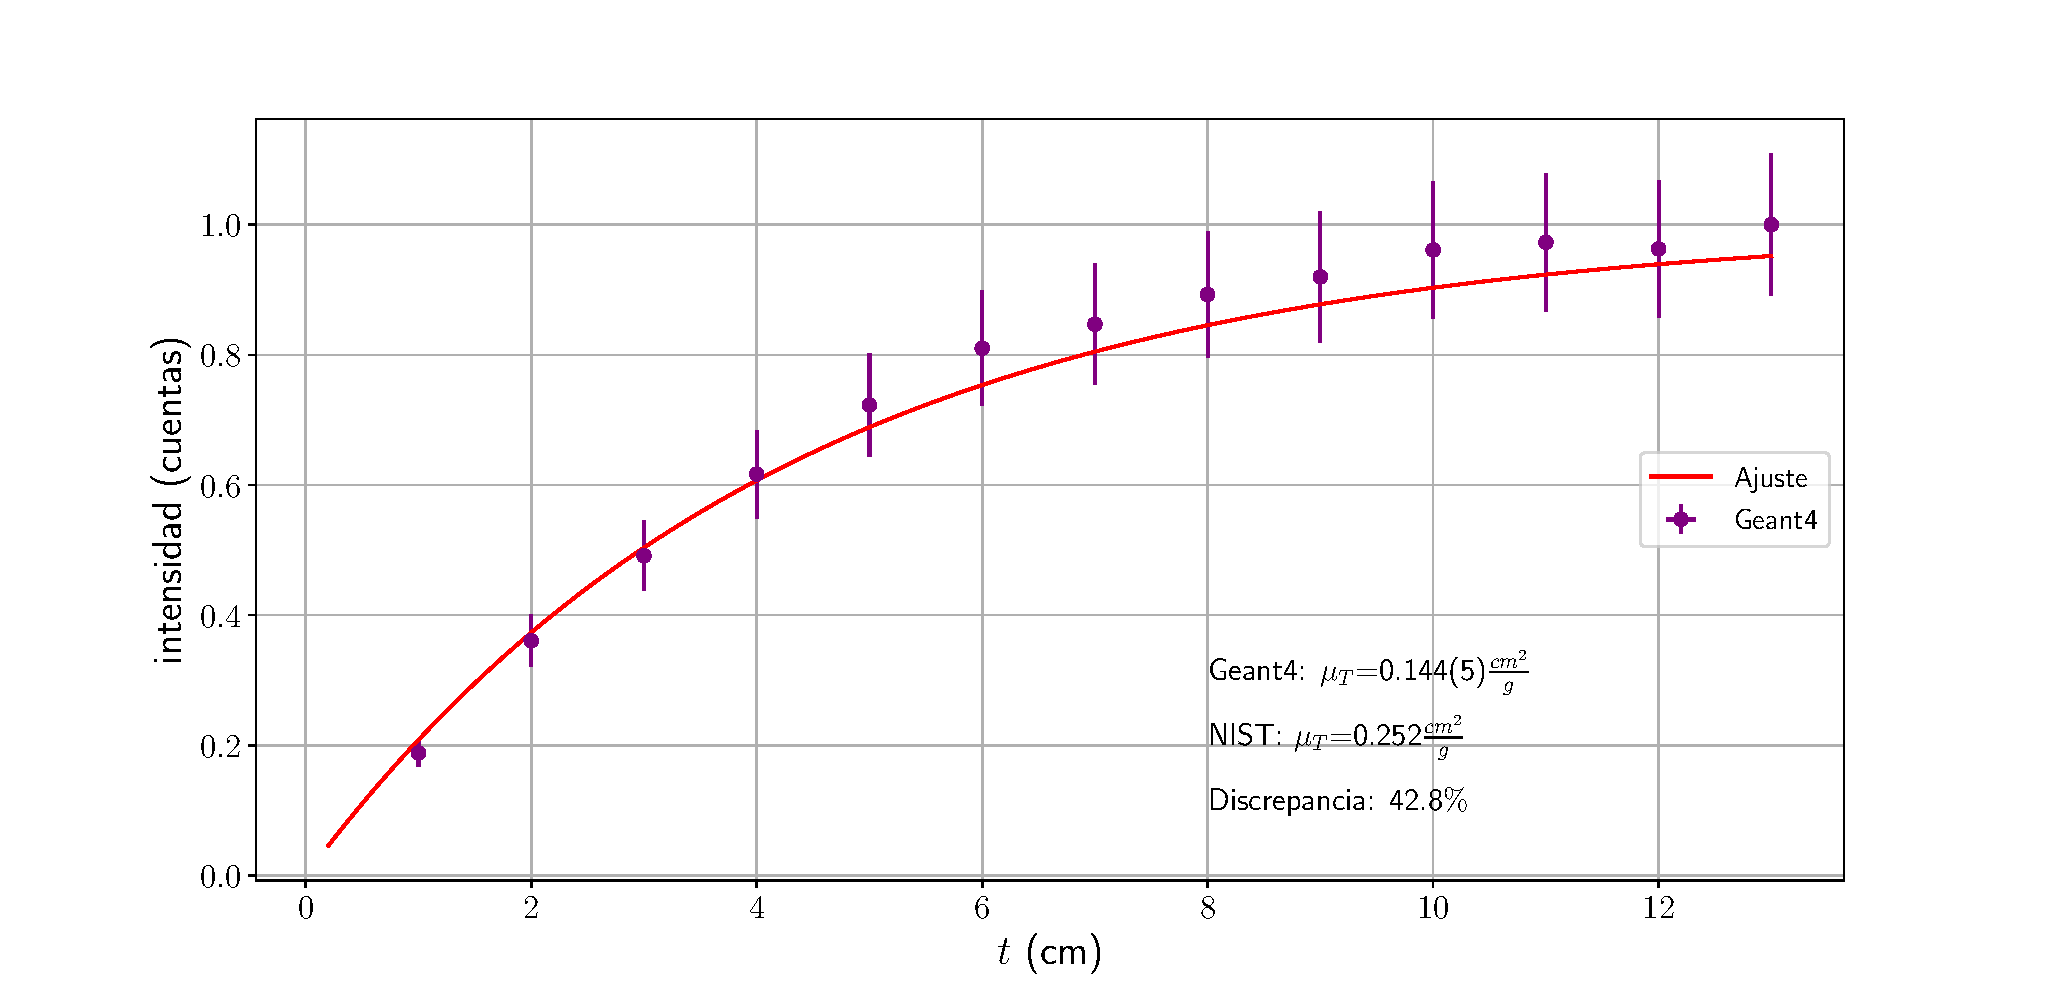
\includegraphics[width=1.0\linewidth]{Kap4/mu_T-m4.pdf}
 	\caption{valores de $\mu_T$. Morteros4.}
 	\label{fig:mut-m4}
 \end{figure}
 
 
 
 
 \section{Morteros 5.}
 
 
 \begin{equation} \label{densidad-mor5}
 \rho=\frac{masa}{volumen}=1.60(6) g/cm^3
 \end{equation}
 
 
 \subsection{Transmisión.}
 
\begin{figure}[H]
	\centering
	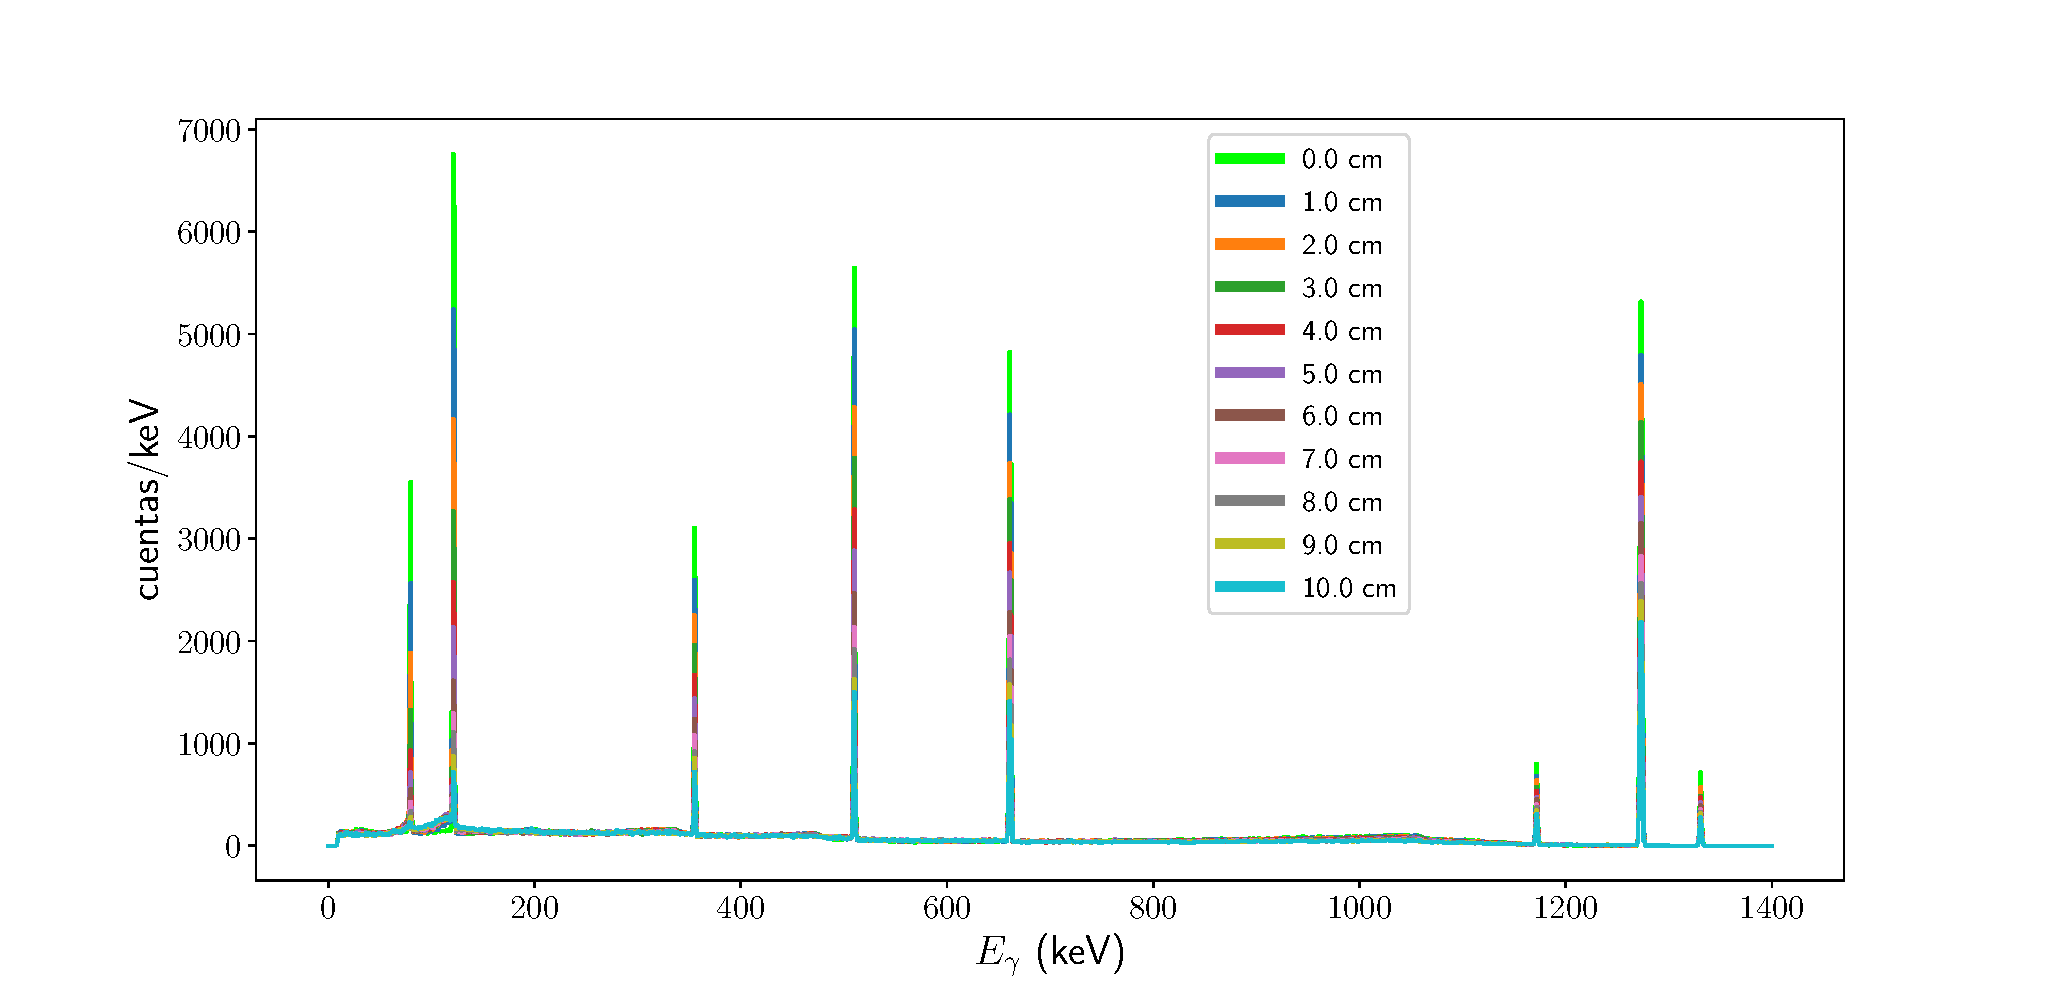
\includegraphics[width=1.0\linewidth]{Kap4/espectro_m5-10Mtrans.pdf}
	\caption{Espectro de 10 láminas de Morteros5. Transmisión}
	\label{fig:espectrom5-10mtrans}
\end{figure}
 
\begin{figure}[H]
	\centering
	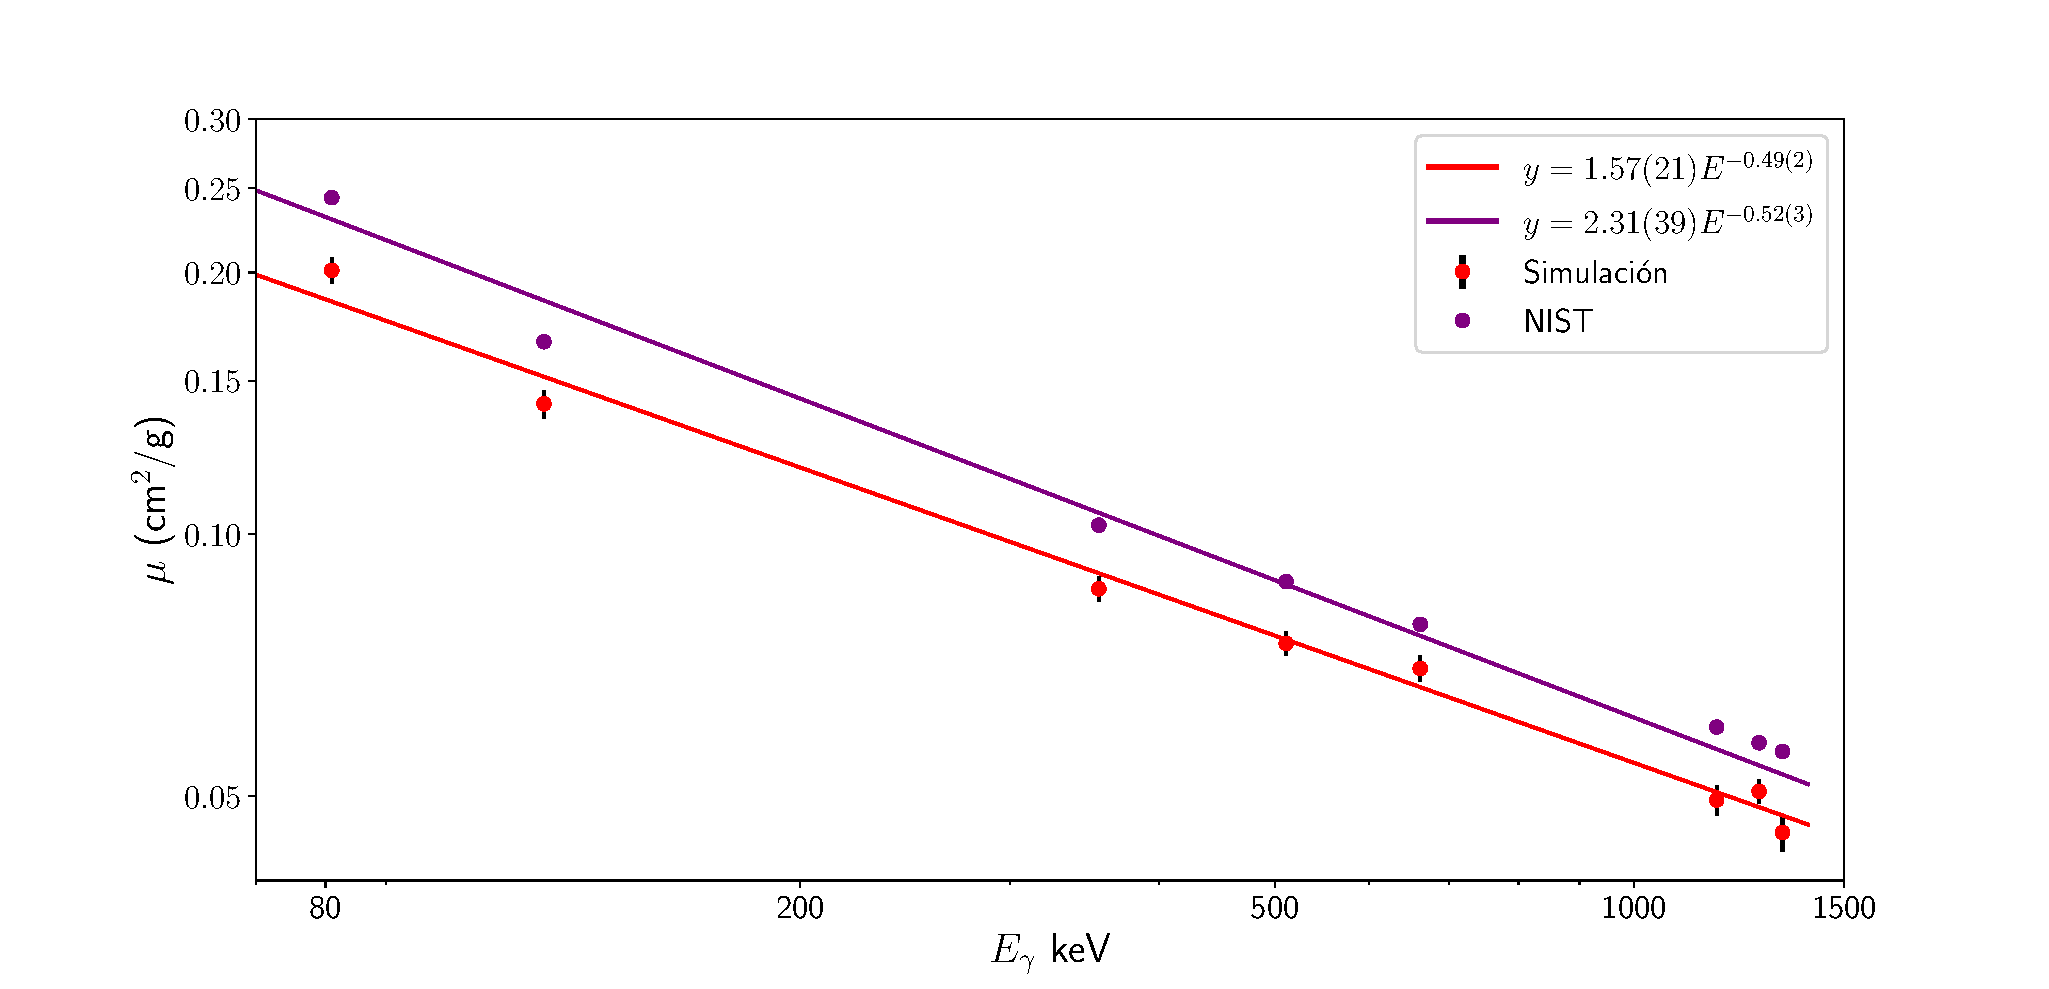
\includegraphics[width=1.0\linewidth]{Kap4/mu-trans-m5.pdf}
	\caption{Ajuste para encontrar $\alpha$ y $n$ a partir de los diferentes $\mu$/$\rho$. Morteros5.}
	\label{fig:mu-trans-m5}
\end{figure}
 
 \subsection{Retrodispersión.}
 
\begin{figure}[H]
	\centering
	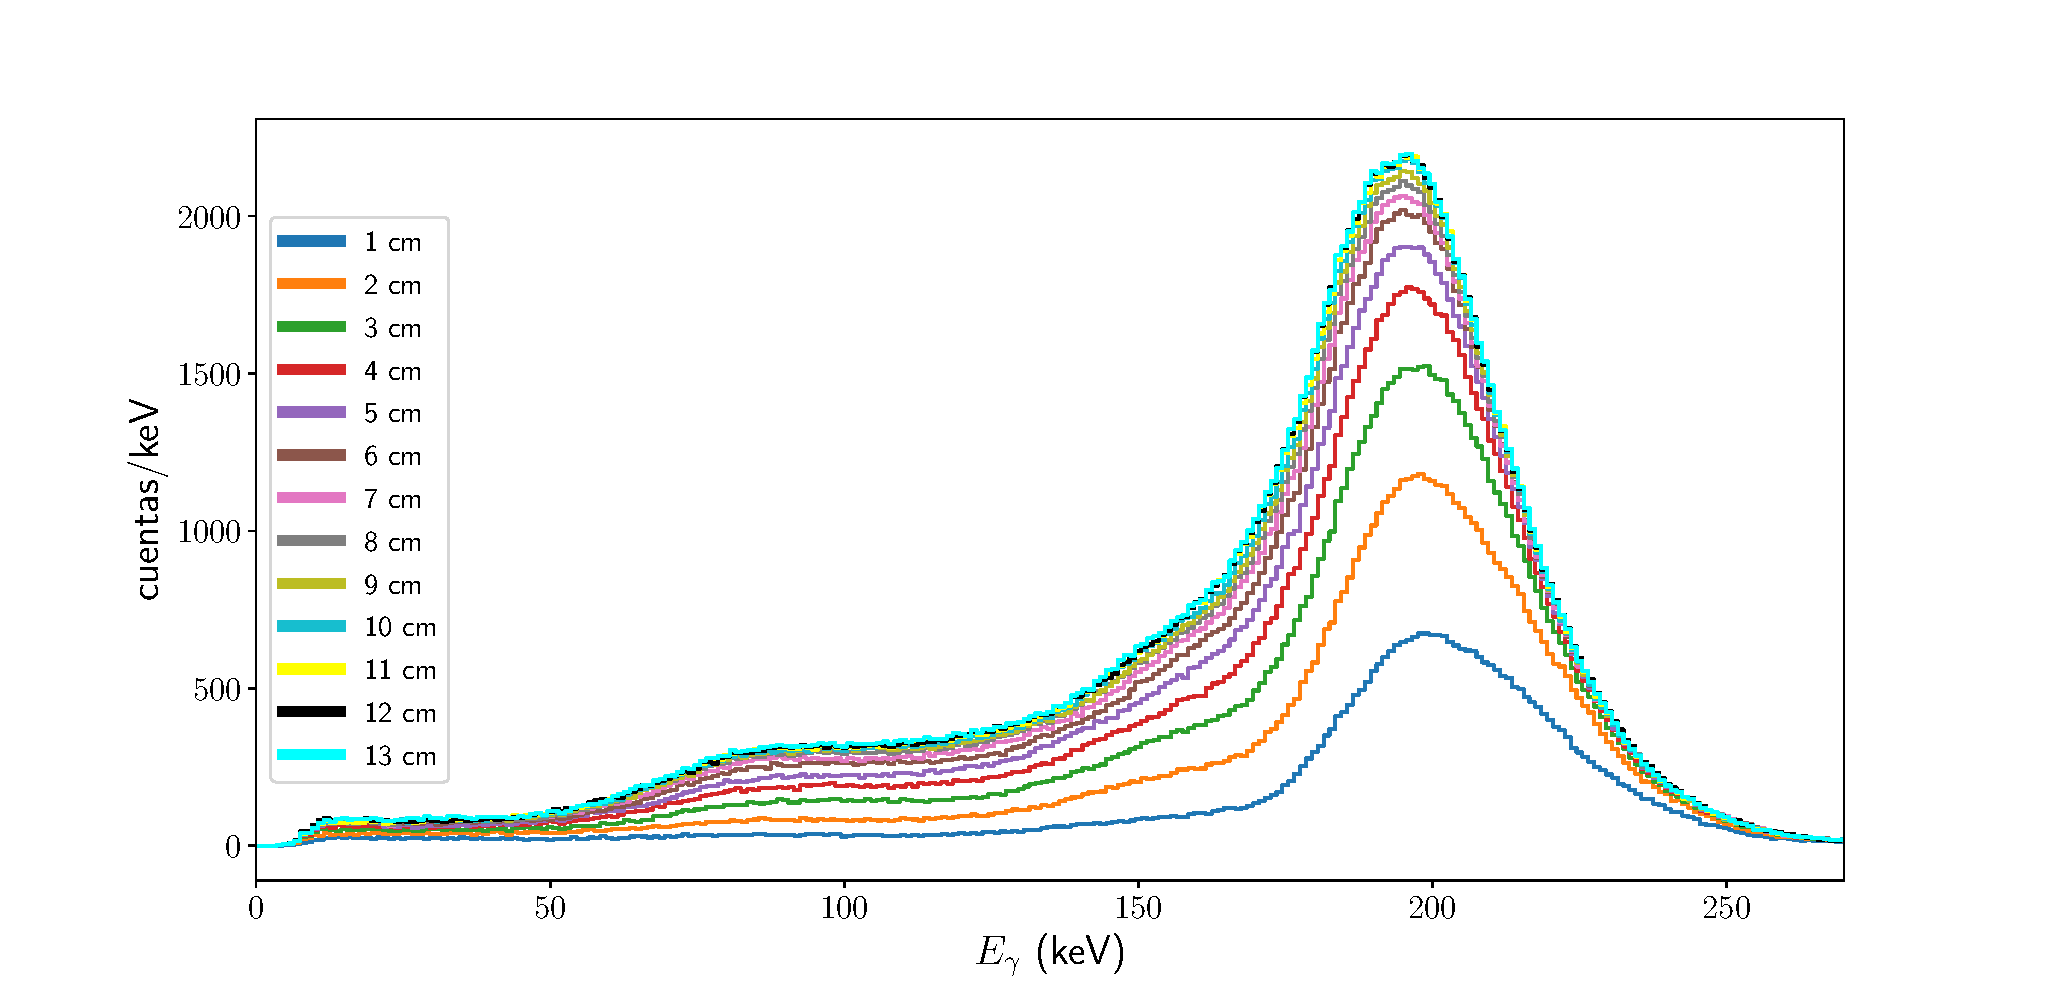
\includegraphics[width=1.0\linewidth]{Kap4/espectro_m5.pdf}
	\caption{Espectro de 10 láminas de Morteros5.}
	\label{fig:espectrom5}
\end{figure}

\begin{figure}[H]
	\centering
	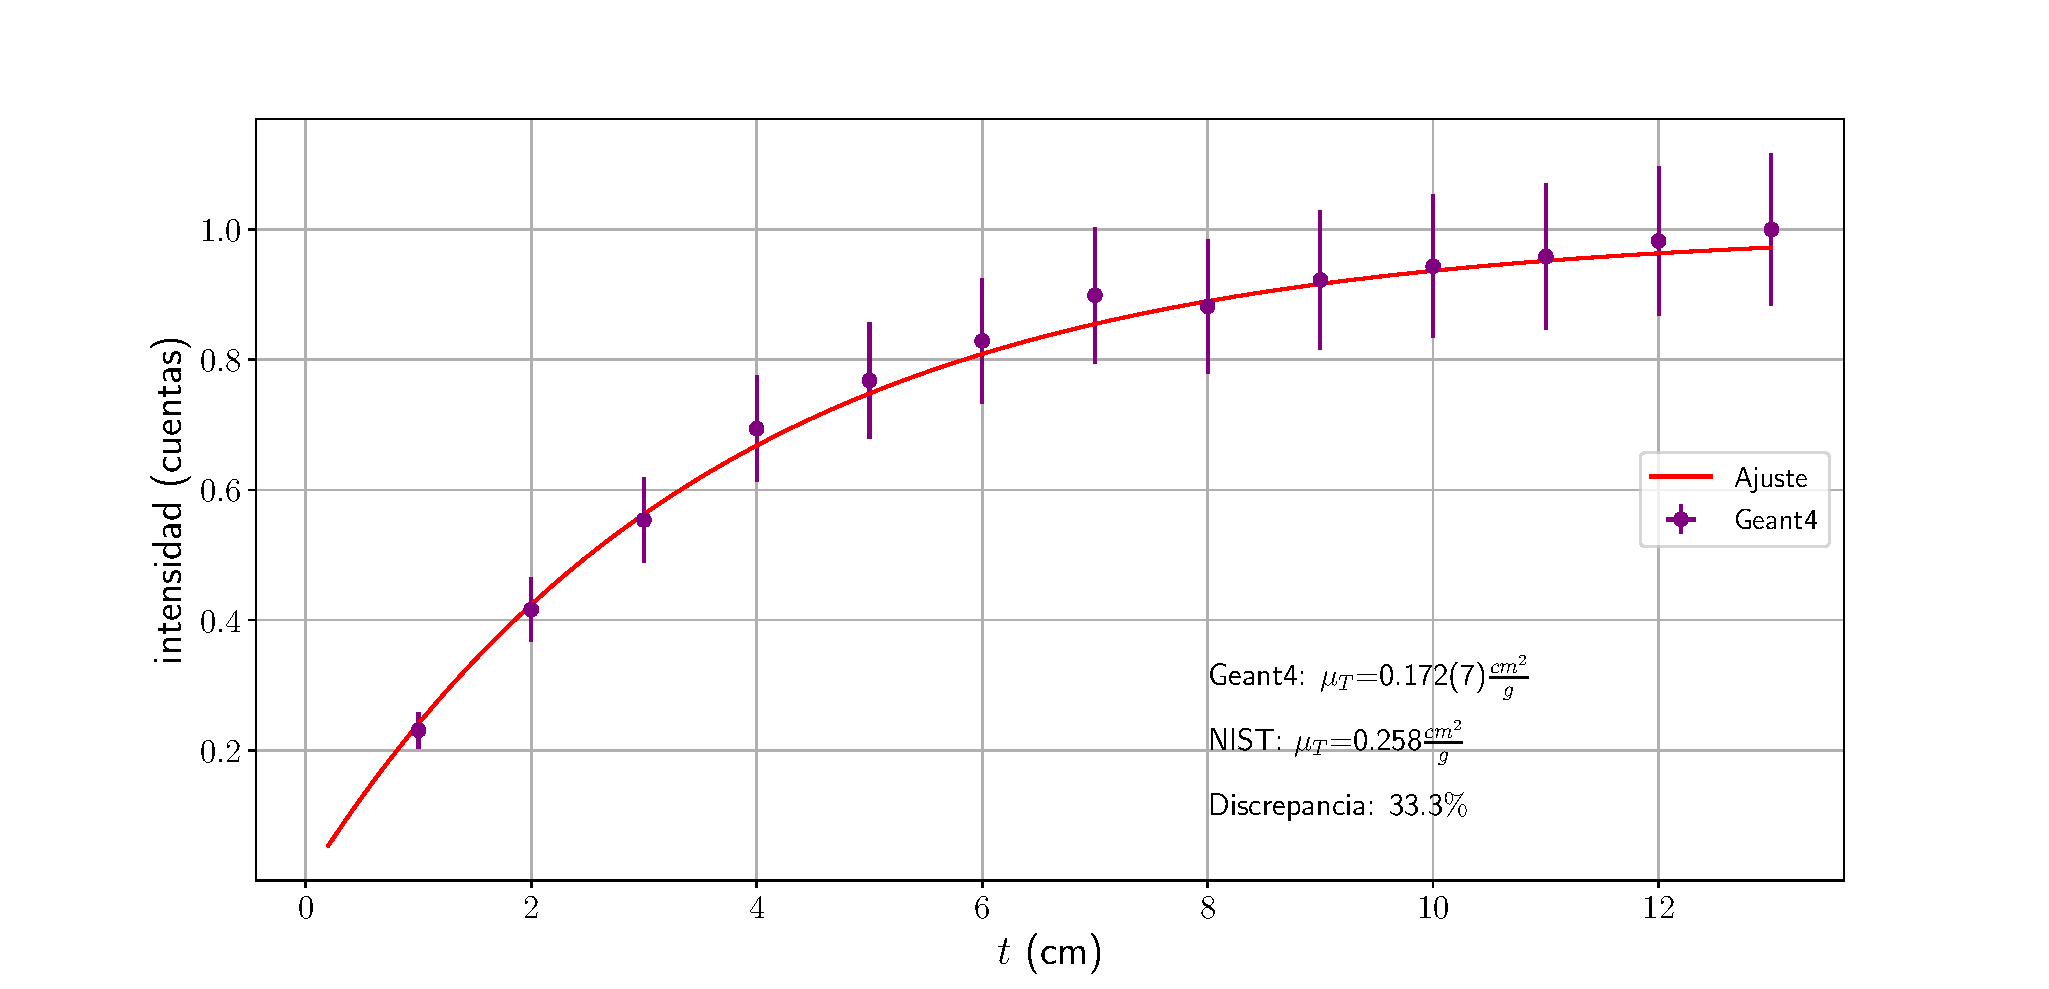
\includegraphics[width=1.0\linewidth]{Kap4/mu_T-m5.pdf}
	\caption{Valores de $\mu_T$. Morteros5.}
	\label{fig:mut-m5}
\end{figure}